\documentclass[12pt,twoside]{book}

\usepackage[utf8]{inputenc}
\usepackage[turkish]{babel}
\usepackage[T1]{fontenc}

\usepackage{amsmath}
\usepackage{amssymb}
\usepackage{amsthm}
\usepackage{enumerate}
\usepackage[most]{tcolorbox}

\usepackage{circuitikz}
\usepackage{cancel}
\usepackage{bodegraph}
\usepackage{gensymb}

\usepackage{verbatim}
\usepackage{listings}
\usepackage{matlab-prettifier}

\usepackage{pgfplots}
\pgfplotsset{compat=newest}
\usepackage{pgffor}
\usepackage{xcolor}

\usepackage{tikz}
\usetikzlibrary{patterns}
\usetikzlibrary{babel}

\usetikzlibrary{shapes.misc}
\tikzset{cross/.style={cross out, draw=black, minimum size=2*(#1-\pgflinewidth), inner sep=0pt, outer sep=0pt},
%default radius will be 3pt. 
cross/.default={3pt}}
\usetikzlibrary{arrows}
\tikzset{
  arrow/.pic={\path[tips,every arrow/.try,->,>=#1] (0,0) -- +(.1pt,0);},
  pics/arrow/.default={triangle 90}
}

\usepackage{siunitx}
\usepackage{textcomp}

\usepackage{hyperref}
\hypersetup{
    colorlinks=true,
    linkcolor=blue,
    filecolor=magenta,      
    urlcolor=cyan,
    pdftitle={Kitap},
    pdfpagemode=FullScreen,
    }

\urlstyle{same}

\usepackage{graphicx}
\graphicspath{{svg-inkscape/}}
\usepackage{geometry}
\usepackage{subcaption}
\usepackage{tabularray}
\usepackage{tabularx}
\DefTblrTemplate{contfoot-text}{default}{Bir sonraki sayfada devam ediyor.} % Uzun Tablolar için alt kısım
\DefTblrTemplate{conthead-text}{default}{(Devam)} % Uzun Tablolar için üst kısım

\usepackage{lscape}

\usepackage{pgfplotstable}
\usepackage{booktabs}

\usepackage{steinmetz}
\usepackage{matlab-prettifier}
\usepackage[tc]{titlepic}


\begin{document}
\shorthandoff{=} % babel paketi hatasını gidermek için gerekli
\renewcommand{\chaptername}{Bölüm}
\renewcommand{\contentsname}{İçindekiler}
\renewcommand{\figurename}{Şekil}
\renewcommand{\tablename}{Çizelge}
\renewcommand{\bibname}{Kaynaklar}
\renewcommand{\listfigurename}{Şekiller}
\renewcommand{\listtablename}{Çizelgeler}
\renewcommand{\appendixname}{Ek}
\renewcommand{\indexname}{Dizin}
\renewcommand{\partname}{Bölüm}
\renewcommand{\proofname}{İspat}
\definecolor{other}{RGB}{171,0,255}

%%%%%%%%%%%%%%%%%%%%%%%%%%%%%%%%%%%%%%%%%%%%%%%%%%%%%%%%%%%%%%%%%%%%%%%%%%%%%%%%%%%
\title{\bfseries{\sc\textcolor{black}{Bilgisayarlı Kontrol Sistemleri \\ Ders Notu}}}
\author{\textcolor{black}{Dr. Mehmet CANEVİ} \\[5pt]
\emph{\textcolor{black}{Bilgisayar Mühendisliği}}\\[2cm]
   \vspace{2cm}
\titlepic{
\includegraphics[width=0.2\textwidth]{logo}\\[5pt]
\textcolor{black}{Niğde Ömer Halisdemir Üniversitesi}\\[5pt]
 \textcolor{black}{Türkiye}\\
 \vfill
 \textcolor{black}{2025}}}
\date{}

\lstset{language=Python, literate={-}{-}1,morekeywords={as,plt,c,np,control}}
\lstset{frame=lines}
\lstset{label={lst:code_direct}}
\lstset{basicstyle=\footnotesize}
\lstset{keepspaces=true}
\lstset{columns=fullflexible}
\lstset{keywordstyle=\color{blue}}
\lstset{commentstyle=\color{green}}
\lstset{stringstyle=\color{red}}
\lstset{showspaces=false}           
\lstset{showstringspaces=false}   

\maketitle
%%%%%%%%%%%%%%%%%%%%%%%%%%%%%%%%%%%%%%%%%%%%%%%%%%%%%%%%%%%%%%%%%%%%%%%%%%%%%%%%%%%
\let \savenumberline \numberline
\def \numberline#1{\savenumberline{#1.}}
\tableofcontents

\documentclass[12pt,hyperref=unicode]{beamer}

\usepackage[utf8]{inputenc}
\usepackage[turkish]{babel}
\usepackage[T1]{fontenc}

\usepackage{amsmath}
\usepackage{amssymb}
\usepackage{amsthm}
\usepackage{enumerate}
\usepackage{tikz}
\usepackage{transparent}
\usepackage{xcolor}
\usepackage{listings}
\usepackage{verbatim}
\usepackage{graphicx}

\usepackage{pgfplots}

\usetheme{Warsaw}
\usecolortheme{default}
\definecolor{nigdeyesili_acik}{RGB}{3, 150, 166}
\definecolor{nigdeyesili_koyu}{RGB}{143, 209, 217}
\setbeamercolor{structure}{fg=nigdeyesili_acik}

\author[Dr. Mehmet CANEVİ]{Arş.~Gör.~Dr.~M.~Canevi\inst{1}}

\institute{
    \inst{1}%
    Bilgisayar Mühendisliği\\
    Mühendislik Fakültesi
}
    
\date[2025] {Ders Notları, Ocak 2025}
\setbeamertemplate{footline}[frame number]

\logo{\transparent{0.4}
\includegraphics[width = 20mm]{logo}}

\definecolor{mGreen}{rgb}{0,0.6,0}
\definecolor{mGray}{rgb}{0.5,0.5,0.5}
\definecolor{mPurple}{rgb}{0.58,0,0.82}
\definecolor{backgroundColour}{rgb}{0.95,0.95,0.92}

\lstloadlanguages{C}
\lstdefinestyle{CStyle}{
    backgroundcolor=\color{backgroundColour},   
    commentstyle=\color{mGreen},
    keywordstyle=\color{red},
    numberstyle=\tiny\color{mGray},
    stringstyle=\color{mGreen},
    basicstyle=\footnotesize,
    breakatwhitespace=false,         
    breaklines=true,                 
    captionpos=b,                    
    keepspaces=true,                 
    numbers=left,                    
    numbersep=2pt,                  
    showspaces=false,                
    showstringspaces=false,
    showtabs=false,                  
    tabsize=1,
    language=C
}
\lstset{style=CStyle}

\AtBeginDocument{\shorthandoff{=}}
\title[Ders 1] {Kod Yazma, Kod Derleme. Değişken Tanımlama, Veri Tipleri. Operatörler.}
\begin{document}
%%%%%%%%%%%%%%%%%%%%%%%%%%%%%%%%%%%%%%%%%%%%%%%%%%%%%%%%%%%%%%%%%%%%%%%%%%%%%%%%
\frame{\titlepage}
\begin{frame}[fragile]{İçidekiler}
    \tableofcontents
\end{frame}
%%%%%%%%%%%%%%%%%%%%%%%%%%%%%%%%%%%%%%%%%%%%%%%%%%%%%%%%%%%%%%%%%%%%%%%%%%%%%%%%
\section{Kod yazma}
\begin{frame}[fragile]{Kod nedir?}
    \begin{itemize}
        \item Bilgisayar tanımı kapsamına giren cihazlara meramımızı anlatmak için yazılan yazıya \textbf{kod} diyebiliriz
        \item Bahsi geçen yazının bir dili olur ve buna kodun dili denir
        \item Bu ders kapsamında \verb|C| dilini kullanacağız
        \item \verb|C| dili insanın anlama şekline daha yakındır
        \item Makinenin anlama şekline yakın diline \textbf{makine dili} denir
    \end{itemize}
\end{frame}
%%%%%%%%%%%%%%%%%%%%%%%%%%%%%%%%%%%%%%%%%%%%%%%%%%%%%%%%%%%%%%%%%%%%%%%%%%%%%%%%
\begin{frame}[fragile]{Derleme nedir?}
    \begin{itemize}
        \item \verb|C| dilinden \textbf{makine dili}ne çeviri işlemidir
        \item Kod yazarken yapılan her güncelleme sonrası derlemeye ihtiyaç duyulur
        \item Derleme bazen hata ile sonuçlanabilir, muhtemel bir \textbf{imla hatası} sebep olabilir
        \item Derleme başarılı olmasına rağmen makine istenen davranışı göstermeyebilir(\textbf{mantıksal hata})
        \item \verb|Windows| için derleme(ve linkleme sonucu) \verb|exe| uzantılı bir dosya üretilir
    \end{itemize}
\end{frame}
%%%%%%%%%%%%%%%%%%%%%%%%%%%%%%%%%%%%%%%%%%%%%%%%%%%%%%%%%%%%%%%%%%%%%%%%%%%%%%%%
\begin{frame}[fragile]{Örnek bir kod}
    Örnek bir kod
    \lstinputlisting{lec1/main.c}
    şeklindedir.
\end{frame}
%%%%%%%%%%%%%%%%%%%%%%%%%%%%%%%%%%%%%%%%%%%%%%%%%%%%%%%%%%%%%%%%%%%%%%%%%%%%%%%%
\begin{frame}[fragile]{Örnek bir makine kodu}
    Örnek bir makine kodu
    \lstinputlisting{lec1/main.o}
    şeklindedir.
\end{frame}
%%%%%%%%%%%%%%%%%%%%%%%%%%%%%%%%%%%%%%%%%%%%%%%%%%%%%%%%%%%%%%%%%%%%%%%%%%%%%%%%
\begin{frame}[fragile]{Makine kodunun temeli}
    $4+6$ işlemini inceleyelim:
    \begin{equation}
        (0100)_2+(0110)_2=(1010)_2=10
    \end{equation}
    1 bitlik en basit toplama işlemi 
    \begin{figure}[!htb]
        \centering
        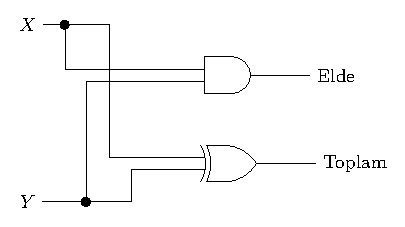
\includegraphics[width=0.5\textwidth]{lec1/xor}
    \end{figure}
    ile gösterilebilir. 4 bit için bu yapı temel alınıp gerçeklenebilir.
\end{frame}
%%%%%%%%%%%%%%%%%%%%%%%%%%%%%%%%%%%%%%%%%%%%%%%%%%%%%%%%%%%%%%%%%%%%%%%%%%%%%%%%
\begin{frame}[fragile]{Makine kodunun temeli(devam)}
    4 bit için bu yapı 
    \begin{figure}[!htb]
        \centering
        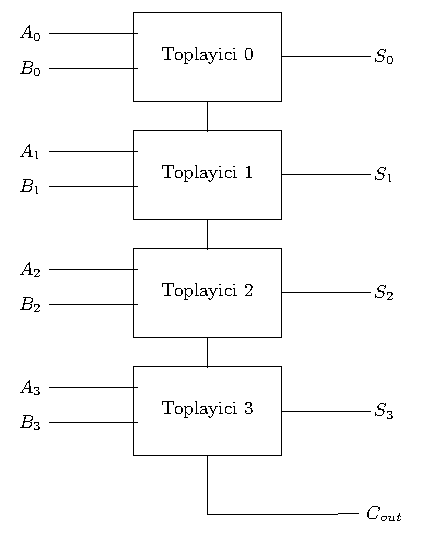
\includegraphics[height=0.6\textheight]{lec1/fulladder}
    \end{figure}
    şeklinde gösterilebilir.
\end{frame}
%%%%%%%%%%%%%%%%%%%%%%%%%%%%%%%%%%%%%%%%%%%%%%%%%%%%%%%%%%%%%%%%%%%%%%%%%%%%%%%%
\begin{frame}[fragile]{Makine kodunun temeli(devam)}
    \begin{itemize}
    \item 4 bitlik toplama devresi \textbf{çıkarma işlemi}, \textbf{çarpma işlemi} vb. işlemler ile aritmetik işlemci oluşturulabilmektedir. 
    \item Mantıksal işlemler için de tasarlanırsa ortaya Aritmetik Lojik Birim(ALB) ortaya çıkmaktadır. 
    \item Merkezi İşlemci Birimi(MİB) denilen karmaşık yapının başlangıcı denebilir.
    \end{itemize}
\end{frame}
%%%%%%%%%%%%%%%%%%%%%%%%%%%%%%%%%%%%%%%%%%%%%%%%%%%%%%%%%%%%%%%%%%%%%%%%%%%%%%%%
\section{Değişken tanımlama ve veri tipleri}
\begin{frame}[fragile]{Değişken isimleri}
    Değişkenler şu şekilde tanımlanmaktadır:
    \begin{lstlisting}
        veri_tipi degisken_adi;
        veri_tipi degisken_adi=ilk_deger;\end{lstlisting}
    Buradaki \lstinline{veri_tipi};
    \begin{itemize}
        \item \lstinline{int} 
        \item \lstinline{float}
        \item \lstinline{double}
        \item \lstinline{char}
    \end{itemize}
     olabilmektedir. \lstinline{degisken_adi} ise 
    \begin{itemize}
     \item türkçe karakter içermemelidir
     \item sadece harf veya alttire ile başlamalıdır
     \item özel karakterler(!,?,vb.) ve boşluk içermemelidir
     \item \lstinline{veri_tipi} anahtar kelimeleri olmamalıdır
    \end{itemize}
    kurallarına uymalıdır.
\end{frame}
%%%%%%%%%%%%%%%%%%%%%%%%%%%%%%%%%%%%%%%%%%%%%%%%%%%%%%%%%%%%%%%%%%%%%%%%%%%%%%%%
\begin{frame}[fragile]{Değişken tiplerinin anlamı}
    Değişkenler
    \begin{itemize}
     \item \lstinline{int} ingilizce \verb|integer| yani tam sayıdan gelmektedir \lstinline{-10,4} gibi
     \item \lstinline{float} ingilizcede kayan noktalı sayı(6-7 basamak) anlamındadır \lstinline{3.14f} gibi
     \item \lstinline{double} ingilizcede iki kat hassasiyet(15 basamak) anlamındadır \lstinline{3.14} gibi
     \item \lstinline{char} ingilizce \verb|character|'den gelir \lstinline{'c','x'} gibi
    \end{itemize}
    veri tipleri ile tanımlanabilmektedir ve 
    \begin{itemize}
        \item \lstinline{int var1=-10;} 
        \item \lstinline{float var2=3.14f;} 
        \item \lstinline{double var3=3.14;} 
        \item \lstinline{char var4='x';} 
    \end{itemize}
    olarak örneklendirilebilir.
\end{frame}
%%%%%%%%%%%%%%%%%%%%%%%%%%%%%%%%%%%%%%%%%%%%%%%%%%%%%%%%%%%%%%%%%%%%%%%%%%%%%%%%
\begin{frame}[fragile]{Çoklu değişken tanımlama}
    Birden fazla değişken
    \begin{itemize}
        \item \lstinline{int a,b,c=-10;} 
        \item \lstinline{float a=2.2,b,c=3.14f;} 
        \item \lstinline{double a,b,c=3.14;} 
        \item \lstinline{char a,b,c;a=b=c='x';}
    \end{itemize}
    şeklinde tanımlanabilir.
\end{frame}
%%%%%%%%%%%%%%%%%%%%%%%%%%%%%%%%%%%%%%%%%%%%%%%%%%%%%%%%%%%%%%%%%%%%%%%%%%%%%%%%
\begin{frame}[fragile]{Değişkenlerin yazdırılması}
    Değişkenler
    \begin{itemize}
        \item \lstinline{int var1=-10;printf("%d",var1);} 
        \item \lstinline{float var2=3.14f;printf("%f",var2);} 
        \item \lstinline{double var3=3.14;printf("%lf",var3);} 
        \item \lstinline{char var4='x';printf("%c",var4);}
        \item \lstinline{printf("%s","Bu bir cumledir.");}
    \end{itemize}
    ile ekrana yazdırılır.
\end{frame}
%%%%%%%%%%%%%%%%%%%%%%%%%%%%%%%%%%%%%%%%%%%%%%%%%%%%%%%%%%%%%%%%%%%%%%%%%%%%%%%%
\begin{frame}[fragile]{Sabit değerli değişkenler}
    Değeri değişmemesi gereken değişkenler
    \begin{itemize}
        \item \lstinline{const int SAAT_DK=60;} 
        \item \lstinline{const float PI_SAYISI=3.14;} 
    \end{itemize}
    şeklinde tanımlanır ve büyük harflerin kullanımı bir gelenektir. Dolayısıyla,
    \begin{itemize}
        \item \lstinline{SAAT_DK=120;} 
        \item \lstinline{PI_SAYISI=5.5;} 
    \end{itemize}
    hata verir.
\end{frame}
%%%%%%%%%%%%%%%%%%%%%%%%%%%%%%%%%%%%%%%%%%%%%%%%%%%%%%%%%%%%%%%%%%%%%%%%%%%%%%%%
\section{Operatörler}
\begin{frame}[fragile]{Matematiksel operatörler}
    Toplama ve çıkarma işlemi
    \begin{itemize}
        \item \lstinline{int a=4+5;int c=a-2;int d=a+c;} 
    \end{itemize}
    ile örneklendirilebilir. Matematiksel operatörler
    \begin{itemize}
        \item \lstinline{+,-} toplama, çıkarma 
        \item \lstinline{*,/} çarpma, bölme
        \item \lstinline{++,--} arttırma, azaltma 
        \item \lstinline{%} \verb|mod| operatörü (bölümden kalan)
        \item \lstinline{=} atama operatörü
    \end{itemize}
    şeklindedir.
\end{frame}
%%%%%%%%%%%%%%%%%%%%%%%%%%%%%%%%%%%%%%%%%%%%%%%%%%%%%%%%%%%%%%%%%%%%%%%%%%%%%%%%
\begin{frame}[fragile]{Matematiksel operatörler(devam)}
    Aşağıdaki operatörler tanımlıdır.
    \begin{itemize}
        \item \lstinline{x+=3;} \lstinline{x=x+3;} 
        \item \lstinline{x-=3;} \lstinline{x=x-3;} 
        \item \lstinline{x*=3;} \lstinline{x=x*3;} 
        \item \lstinline{x/=3;} \lstinline{x=x/3;} 
        \item \lstinline{x%=3;} \lstinline{x=x%3;} 
    \end{itemize}
\end{frame}
%%%%%%%%%%%%%%%%%%%%%%%%%%%%%%%%%%%%%%%%%%%%%%%%%%%%%%%%%%%%%%%%%%%%%%%%%%%%%%%%
\begin{frame}[fragile]{Karşılaştırma operatörleri}
    Aşağıdaki operatörler ile karşılaştırma başarılı ise 1 değilse sıfır değerini alır.
    \begin{itemize}
        \item \lstinline{x>y} Büyüktür
        \item \lstinline{x>=y} Büyük eşittir
        \item \lstinline{x<y} Küçüktür
        \item \lstinline{x<=y} Küçük eşittir
        \item \lstinline{x==y} Eşittir
        \item \lstinline{x!=y} Eşit değildir
    \end{itemize}
\end{frame}
%%%%%%%%%%%%%%%%%%%%%%%%%%%%%%%%%%%%%%%%%%%%%%%%%%%%%%%%%%%%%%%%%%%%%%%%%%%%%%%%
\begin{frame}[fragile]{Mantıksal operatörleri}
    Mantıksal operatörler
    \begin{itemize}
        \item \lstinline{sart1 && sart2} VE
        \item \lstinline{sart1 || sart2} VEYA 
        \item \lstinline{!sart} DEĞİLDİR 
    \end{itemize}
    olarak verilmiştir.
\end{frame}
%%%%%%%%%%%%%%%%%%%%%%%%%%%%%%%%%%%%%%%%%%%%%%%%%%%%%%%%%%%%%%%%%%%%%%%%%%%%%%%%
\end{document}
\chapter{Ayrıklaştırma}
Türevin geometrik yorumu 
\begin{equation}
    \frac{dy(t)}{dt}\approx\frac{\Delta y}{\Delta t}
\end{equation}
olmak üzere
\begin{equation}
\begin{split}
    \frac{dy(t)}{dt}&\approx\frac{\Delta y}{\Delta t}\\
    &\approx\frac{y((k+1)T)-y(kT)}{(k+1)T-kT}\\
    &\approx\frac{y((k+1)T)-y(kT)}{T}
\end{split}
\end{equation}
elde edilir. Ayrık bir sinyalin türevi ardışık değerler farkının örnekleme zamanına oranı ile hesaplanabilmektedir. Örneğin, $y(kT)=\sin(kT)$ ve $T=0.1$ olmak üzere
\begin{equation}
    \frac{y((k+1)T)-y(kT)}{T}=10(\sin((k+1)0.1)-\sin(0.1k))
\end{equation}
ve dolayısıyla
\begin{equation}
\begin{split}
    \{10\sin(0.1),10(\sin(0.2)-\sin(0.1)),10(\sin(0.3)-\sin(0.2)),\cdots\}\\
    \{0.9983,0.9884, 0.9685,\cdots\}
\end{split}
\end{equation}
elde edilir. $y(kT)=\sin(kT)$ sinyalinin türevinin $\frac{d\sin(t)}{dt}=\cos(t)$ olduğu bilindiğinden
\begin{equation}
    \begin{split}
        \{cos(0.1),cos(0.2),cos(0.3),\cdots\}\\
        \{ 0.9950,0.9801,0.9553,\cdots\}
    \end{split}
\end{equation}
elde edilir ve ayrık türev ile benzer değerler olduğu görülmektedir. Bu yaklaşıklığın türeve yakınsaması için örnekleme zamanı $T$ daha küçük seçilmelidir. 
\begin{equation}
    \frac{dq(t)}{dt}=x
\end{equation}
olmak üzere
\begin{equation}
\begin{split}
    \frac{dq(t)}{dt}&=x\\
    dq(t)&=xdt\\
    \int dq(t)&=\int xdt\\
    q(t)&=\int xdt
\end{split}
\end{equation}
elde edilir. Buradan hareketle,
\begin{equation}
    \begin{split}
        \frac{\Delta q}{\Delta t}&=x\\
        \frac{q((k+1)T)-q(kT)}{(k+1)T-kT}&=x\\
        \frac{q((k+1)T)-q(kT)}{T}&=x\\
        q((k+1)T)-q(kT)&=xT\\
        q((k+1)T)&=q(kT)+xT
    \end{split}
\end{equation}
ifadesi bulunur. Ayrık zamanda integral birikimli toplama karşılık gelmektedir. Bu karşılıklar Zero Order Hold(ZOH) ile elde edilmiştir. ZOH örnekleme zamanı boyunca değerlerin sabit olduğu varsayımına dayanmaktadır. Bu durum
\begin{equation}
    x(t)=x(kT),\quad kT\leq t\leq (k+1)T
\end{equation}
ile ifade edilebilir. ZOH için transfer fonksiyonu elde etmek amacıyla girişe $\delta(t)$ birim darbe fonksiyonu uygulanırsa çıkışında $u(t)-u(t-T)$ elde edilir. Bu durumda S tanım bölgesinde çıkış ifadesi
\begin{equation}
\begin{split}
    \mathcal{L}\{u(t)-u(t-T)\}&=\mathcal{L}\{u(t)\}-\mathcal{L}\{u(t-T)\}\\
    &=\mathcal{L}\{u(t)\}-e^{-sT}\mathcal{L}\{u(t)\}\\
    &=\frac{1}{s}-e^{-sT}\frac{1}{s}\\
    &=(1-e^{-sT})\frac{1}{s}
\end{split}
\end{equation}
şeklindedir. ZOH transfer fonksiyonu ile bir $G(s)$ sistemi birlikte Z dönüşümü yapılmalıdır. Örneğin,
\begin{equation}
    G(s)=\frac{1}{s+1}
    \label{eqn:ornek_sistem}
\end{equation}
sistemi ayrıklaştırılmak istensin. Bu durumda $G_{ZOH}(s)G(s)$ ayrıklaştırılmalıdır. Bu sebeple,
\begin{equation}
    L(s)=G_{ZOH}(s)G(s)=\frac{1-e^{-sT}}{s(s+1)}
\end{equation}
ifadesi Z tanım bölgesine
\begin{equation}
\begin{split}
    \mathcal{Z}\{L(s)\}&=\mathcal{Z}\left\{\frac{1-e^{-sT}}{s(s+1)}\right\}\\
    &=\mathcal{Z}\{1-e^{-sT}\} \mathcal{Z}\left\{\frac{1}{s(s+1)} \right\}\\
    &=(1-z^{-1}) \left(\mathcal{Z}\left\{\frac{1}{s}-\frac{1}{s+1} \right\}\right)\\
    &=\left(1-\frac{1}{z}\right) \left(\mathcal{Z}\left\{\frac{1}{s}\right\}-\mathcal{Z}\left\{\frac{1}{s+1} \right\}\right)\\
    &=\frac{z-1}{z} \left(\frac{z}{z-1}-\frac{z}{z-e^{-1}}\right)\\
    &=\left(1-\frac{z-1}{z-e^{-1}}\right)\\
    &=\frac{1-e^{-1}}{z-e^{-1}}
\end{split}\label{eqn:ornek_sistem_zoh}
\end{equation}
olarak dönüştürülür.

First Order Hold(FOH) yöntemi ise
\begin{equation}
    x(t)=x(kT)+\frac{t-kT}{T}(x((k+1)T)-x(kT)),\quad kT\leq t\leq (k+1)T
\end{equation}
olarak tanımlanır. Eşitliğin sağ tarafı $t=kT$ için $x(kT)$, $t=(k+0.5)T$ için 
\begin{equation}
\begin{split}
    x(t)&=x(kT)+\frac{t-kT}{T}(x((k+1)T)-x(kT)),\quad kT\leq t\leq (k+1)T\\
    &=x(kT)+\frac{kT+0.5T-kT}{T}(x((k+1)T)-x(kT))\\
    &=x(kT)+0.5(x((k+1)T)-x(kT))\\
    &=x(kT)+0.5x((k+1)T)-0.5x(kT)\\
    &=0.5x((k+1)T)+0.5x(kT)
\end{split}
\end{equation}
ve $t=(k+1)T$ için ise 
\begin{equation}
    \begin{split}
        x(t)&=x(kT)+\frac{t-kT}{T}(x((k+1)T)-x(kT)),\quad kT\leq t\leq (k+1)T\\
        x(t)&=x(kT)+\frac{(k+1)T-kT}{T}(x((k+1)T)-x(kT))\\
        x(t)&=x(kT)+x((k+1)T)-x(kT)\\
        x(t)&=x((k+1)T)
    \end{split}
\end{equation}
olarak elde edilir. Görüldüğü üzere ZOH yönteminin aksine $T$ süre boyunca değerler değişmektedir. FOH için birim darbe yanıtı
\begin{equation}
    x(t)=\begin{cases}
        t+\frac{1}{T} & 0\leq t\leq \frac{1}{T}\\
        -t+\frac{1}{T} & \frac{1}{T}\leq t\leq \frac{2}{T}\\
        0 & t>\frac{2}{T}
    \end{cases}
\end{equation}
ve işlem kolaylığı açısından $T=1$ alınırsa 
\begin{equation}
    x(t)=(1-t)u(2-t)+2tu(1-t)
\end{equation}
şeklindedir. S dönüşümü sonucu
\begin{equation}
\begin{split}
    \mathcal{L}\{x(t)\}&=\mathcal{L}\{(1-t)u(2-t)\}+\mathcal{L}\{2tu(1-t)\}\\
    &=\mathcal{L}\{(1-t)(1-u(t-2))\}+\mathcal{L}\{2t(1-u(t-1))\}\\
    &=\mathcal{L}\{(1-t)\}-\mathcal{L}\{(1-t)u(t-2)\}+\mathcal{L}\{2t\}-\mathcal{L}\{2tu(t-1)\}\\
    &=\mathcal{L}\{(1+t)\}+\mathcal{L}\{(t-1)u(t-2)\}-\mathcal{L}\{2tu(t-1)\}\\
    &=\mathcal{L}\{(1+t)\}+\mathcal{L}\{(t-1)u(t-2)\}-\mathcal{L}\{(2t-2+2)u(t-1)\}\\
    &=\mathcal{L}\{(1+t)\}+\mathcal{L}\{(t-1-1+1)u(t-2)\}-\mathcal{L}\{(2t-2+2)u(t-1)\}\\
    &=\mathcal{L}\{(1+t)\}+\mathcal{L}\{(t-2)u(t-2)+u(t-2)\}-\mathcal{L}\{(2t-2)u(t-1)+2u(t-1)\}\\
    &=\frac{1}{s}+\frac{1}{s^2}+\frac{e^{-2s}}{s^2}+\frac{e^{-2s}}{s}-2\frac{e^{-s}}{s^2}-\frac{2e^{-s}}{s}\\
    &=\frac{1-2e^{-s}+e^{-2s}}{s}+\frac{1-2e^{-s}+e^{-2s}}{s^2}\\
    &=\frac{(1-e^{-s})^2}{s}+\frac{(1-e^{-s})^2}{s^2}\\
    &=\frac{(1-e^{-s})^2}{s^2}(s+1)\\
\end{split}
\end{equation}
elde edilir. FOH için transfer fonksiyonu
\begin{equation}
    \begin{split}
        G_{FOH}(s)&=\frac{(1-e^{-s})^2}{T^2s^2}\frac{Ts+1}{T}\\
        &=G_{ZOH}^2(s)\frac{Ts+1}{T}
\end{split}
\end{equation}
şeklindedir. Örneğin daha önce Denklem~\ref{eqn:ornek_sistem} ile verilen sistemi FOH yöntemi ve yine aynı örnekleme zamanı ile ayrıklaştırmak gerekirse
\begin{equation}
\begin{split}
    L(s)&=\frac{1}{s+1}G_{FOH}(s)\\
    &=\frac{1}{s+1}\frac{(1-e^{-s})^2}{T^2s^2}\frac{Ts+1}{T}\\
    &=\frac{1}{s+1}\frac{(1-e^{-s})^2}{s^2}(s+1)\\
    &=\frac{(1-e^{-s})^2}{s^2}
\end{split}
\end{equation}
ifadesi Z dönüşümüne tabi tutulmalıdır. Dolayısıyla,
\begin{equation}
    \begin{split}
        G(z)&=\mathcal{Z}\left\{\frac{(1-e^{-s})^2}{s^2}\right\}\\
        &=\mathcal{Z}\{(1-e^{-s})^2\}\mathcal{Z}\left\{\frac{1}{s^2}\right\}\\
        &=\left(1-z^{-1}\right)^2\frac{Tz}{(z-1)^2}\\
        &=\left(\frac{z-1}{z}\right)^2\frac{z}{(z-1)^2}\\
        &=\frac{1}{z}
    \end{split}\label{eqn:ornek_sistem_foh}
\end{equation}
elde edilir. Görüldüğü üzere, birim gecikme elde edilmiştir.

\begin{enumerate}
    \item $x(t)=sin(t)$ fonksiyonunun türevini hesaplayıp çiziniz.
    \begin{lstlisting}[style=Matlab-editor]
    t=0:0.1:10;
    xt=sin(t);
    dxt=zeros(size(t));
    T=t(2)-t(1);
    for i=2:length(t)
        dxt(i)=(xt(i)-xt(i-1))/T;
    end
    figure(1);clf;hold on;grid on;xlabel("Zaman(s)");ylabel("x(t)");title("sin(t) ve turevi");
    plot(t,xt,'k','LineWidth',2);
    plot(t,dxt,'r','LineWidth',2);
    \end{lstlisting}
    Şekil~\ref{fig:lec2_plot1}'de $sin(t)$ ve türevi gösterilmiştir.
    \begin{figure}[!htb]
        \centering
        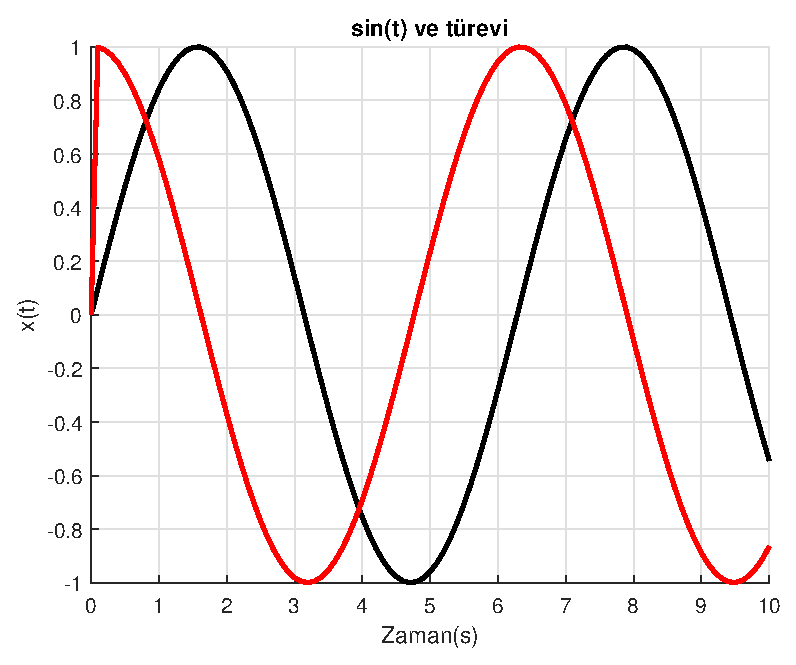
\includegraphics[width=0.5\textwidth]{img/lec2_plot1}
        \caption{$sin(t)$ ve türevinin karşılaştırılması($T=0.1$)}
        \label{fig:lec2_plot1}
    \end{figure}

    Şekil~\ref{fig:lec2_plot2}'de daha düşük bir örnekleme zamanı seçilmiştir ve bu sebeple gerek sinyal gerekse türevi düşük kalitededir.
    \begin{figure}[!htb]
        \centering
        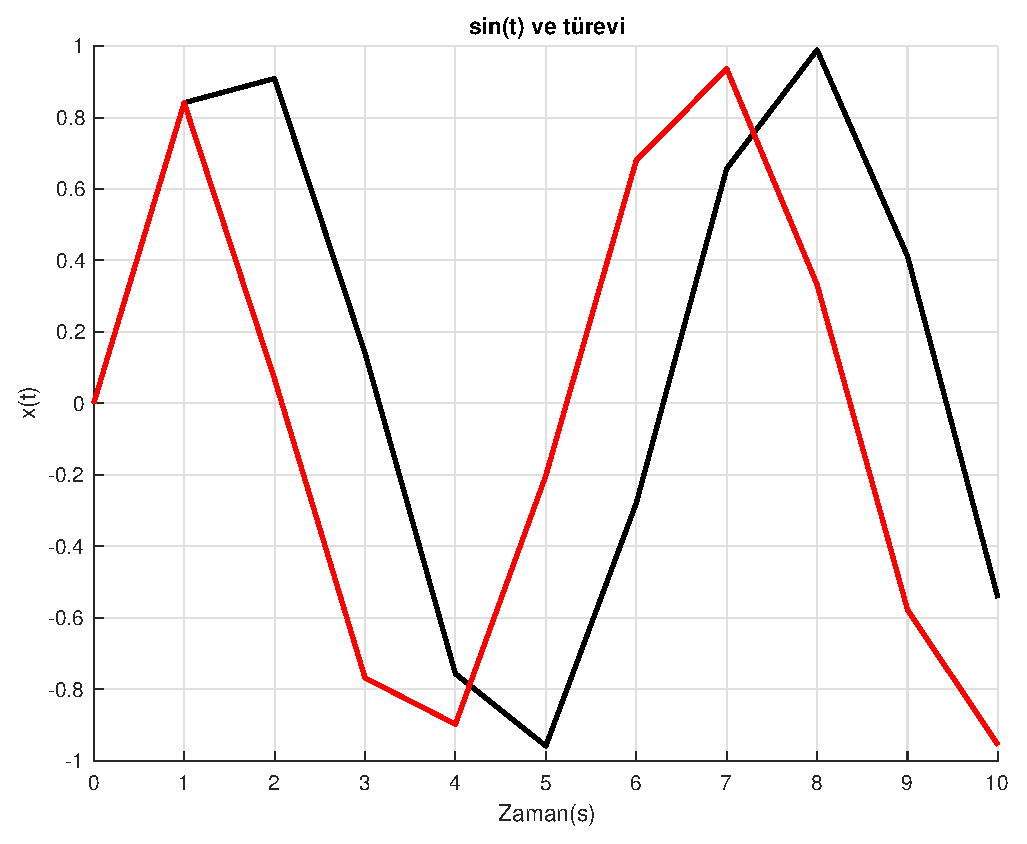
\includegraphics[width=0.5\textwidth]{img/lec2_plot2}
        \caption{$sin(t)$ ve türevinin karşılaştırılması($T=1$)}
        \label{fig:lec2_plot2}
    \end{figure}
    \item $x(t)=e^{-t}$ sinyalinin integralini hesaplayınız ve çizdiriniz.
    \begin{lstlisting}[style=Matlab-editor]
    t=0:1:10;
    xt=exp(-t);
    q=zeros(size(t));
    T=t(2)-t(1);
    for i=2:length(t)
        q(i)=q(i-1)+xt(i-1)*T;
    end
    figure(1);clf;hold on;grid on;xlabel("Zaman(s)");ylabel("x(t)");title("sin(t) ve integrali");
    plot(t,xt,'k','LineWidth',2);
    plot(t,q,'r','LineWidth',2);
    \end{lstlisting}
    Şekil~\ref{fig:lec2_plot3}'de integral çizdirilmiştir.
    \begin{figure}[!htb]
        \centering
        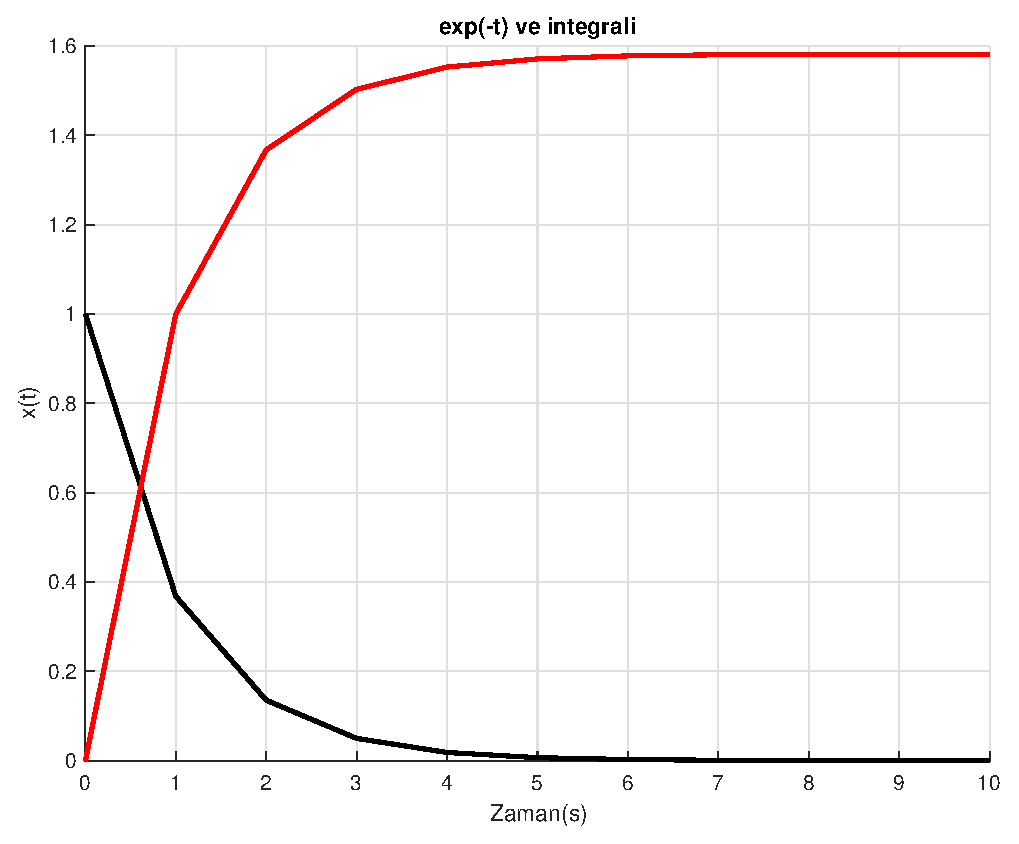
\includegraphics[width=0.5\textwidth]{img/lec2_plot3}
        \caption{$sin(t)$ ve integralinin karşılaştırılması($T=1$)}
        \label{fig:lec2_plot3}
    \end{figure}
    \item ZOH yöntemini kullanarak $T=1$ olmak üzere $x(kT)=1$ sinyalini veri tutucunu çıkışını çizdiriniz.
    \begin{lstlisting}[style=Matlab-editor]
    T=1;
    t=0:T:3;
    xt=[1,2,-1,3];
    
    tnew=0:0.01:4;
    yt=zeros(size(tnew));
    for i=1:length(t)
        for j=1:100
            yt(100*(i-1)+j)=xt(i);
        end
    end
    figure(1);clf;hold on;grid on;xlabel("Zaman(s)");ylabel("x(t)");title("ZOH ornegi");
    stem(t,xt,'k','LineWidth',2);
    plot(tnew,yt,'r','LineWidth',2);
    \end{lstlisting}
    Şekil~\ref{fig:lec2_plot4}'de ZOH işleminin sonucu gösterilmiştir.
    \begin{figure}[!htb]
        \centering
        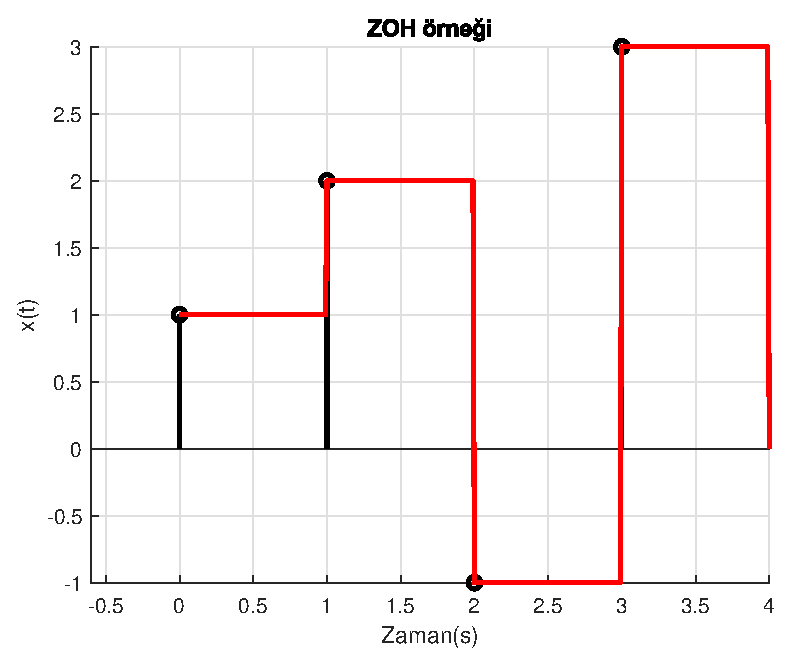
\includegraphics[width=0.5\textwidth]{img/lec2_plot4}
        \caption{ZOH örneği}
        \label{fig:lec2_plot4}
    \end{figure}
\end{enumerate}
\chapter{Fark Denklemleri}
Örnek sistemin ZOH yöntemi ile elde edilen ve Denklem~\ref{eqn:ornek_sistem_zoh} ile verilen sistem için
\begin{equation}
\begin{split}
    G_{ZOH}(z)&=\frac{1-e^{-1}}{z-e^{-1}}\\
    &=\frac{(1-e^{-1})z^{-1}}{1-e^{-1}z^{-1}}\\
    \frac{y(z)}{u(z)}&=\frac{(1-e^{-1})z^{-1}}{1-e^{-1}z^{-1}}\\
    y(z)(1-e^{-1}z^{-1})&=\frac{(1-e^{-1})z^{-1}u(z)}{1-e^{-1}z^{-1}}\\
    y(z)-y(z-1)e^{-1}&=(1-e^{-1})u(z-1)\\
    y(z)&=y(z-1)e^{-1}+(1-e^{-1})u(z-1)\\
    y(z)&=0.3679y(z-1)+0.6321u(z-1)
\end{split}
\end{equation}
elde edilir. Z tanım bölgesinde tanımlı transfer fonksiyonundan fark denklemine geçişe örnektir. Fark denklemleri programlama dilleri ile kolaylıkla gerçeklenebilmektedir.
\begin{lstlisting}
u=ones(1,length(t));
y=zeros(1,length(t));

for i=2:length(t)
    y(i)=exp(-T)*y(i-1)+(1-exp(-T))*u(i);
end\end{lstlisting}
Benzer şekilde FOH yöntemi ile elde edilen ve Denklem~\ref{eqn:ornek_sistem_foh} ile verilen ifade için
\begin{equation}
    \begin{split}
        G_{FOH}(z)&=\frac{1}{z}\\
        \frac{y(z)}{u(z)}&=z^{-1}\\
        y(z)&=u(z-1)
    \end{split}
\end{equation}
elde edilir.
Yay-Kütle-Damper sistemi için dinamikleri ifade eden denklem
\begin{equation}
    m\ddot{x}(t)+b\dot{x}(t)+kx(t)=u(t)
\end{equation}
olarak verilmiştir. Bu diferansiyel denklem S tanım bölgesine dönüştürülürse
\begin{equation}
\begin{split}
    ms^2X(s)+b sX(s)+kX(s)&=U(s)\\
    (ms^2+b s+k)X(s)&=U(s)\\
    \frac{X(s)}{U(s)}=\frac{1}{ms^2+b s+k}
\end{split}
\end{equation}
elde edilir.
\chapter{Zaman Domeni Kriterleri}
Sürekli zamanda tanımlı birinci dereceden bir transfer fonksiyonu
\begin{equation}
    G(s)=\frac{p}{s+p}\label{eqn:1storder_sys}
\end{equation}
olarak verilsin. Birim basamak giriş için yanıt
\begin{equation}
\begin{split}
    y(t)&=\mathcal{L}^{-1}\left\{\frac{p}{s+p}\cdot\frac{1}{s}\right\}\\
    &=\mathcal{L}^{-1}\left\{\frac{1}{s}\right\}-\mathcal{L}^{-1}\left\{\frac{1}{s+p}\right\}\\
    &=1-e^{-pt}
\end{split}
\end{equation}
şeklinde hesaplanır. $e^{-t}$ fonksiyonunun aldığı değerler için Çizelge~\ref{tbl:exp_func} verilmiştir.
% \setlength{\tabcolsep}{40pt}
\begin{table}[!htb]
    \centering
    \caption{$e^{-t}$ fonksiyonunun aldığı değerler}
    \label{tbl:exp_func}
    \begin{tabularx}{\textwidth}{ccc}\hline
        Zaman $t(s)$& Değer $e^{-t}$& $1-e^{-t}$\\[5pt]\hline
        $1$& $0.3679$& $0.6321$\\[5pt]
        $2$& $0.1353$& $0.8647$\\[5pt]
        $3$& $0.0498$& $0.9502$\\[5pt]
        $4$& $0.0183$& $0.9817$\\[5pt]
        $5$& $0.0067$& $0.9933$\\[5pt]
        $6$& $0.0025$& $0.9975$\\[5pt]\hline
    \end{tabularx}
\end{table}
Görüldüğü üzere \ref{eqn:1storder_sys} ile verilen sistemin yanıtı $p$ değişkeninin değerinden bağımsız olarak $1$ değerine yakınsamaktadır. $1$ değerini aşmamaktadır. Dolayısıyla aşım değeri $\%0$'dır. Sürekli halde oturduğu değerin $\%2$ altı veya üstü ile tanımlanan $\%2$'lik banda çıkmamak üzere girdiği zamana yerleşme zamanı denir. Bu tanımdan ve Çizelge~\ref{tbl:exp_func}'den yola çıkarak \ref{eqn:1storder_sys} ile verilen sistemin yerleşme zamanı $t_s=4\,s$'dir. $p=1$ olmaması durumunda zaman ekseni genişler veya daralır bu sebepten yerleşme zamanı 
\begin{equation} 
    t_s=\frac{4}{p}
\end{equation} 
ile hesaplanır. İkinci dereceden bir sistem
\begin{equation}
    G(s)=\frac{w_n^2}{s^2+2\zeta w_ns+w_n^2}
\end{equation}
ile tanımlanmaktadır. Burada $\zeta$ sönüm oranı ve $w_n$ doğal frekans olarak adlandırılmaktadır. İkinci dereceden polinomun kökleri bulunurken faydalanılan $\Delta=b^2-4ac$ hesaplanırsa,
\begin{equation}
\begin{split}
    \Delta&=(2\zeta w_n)^2-4 w_n^2\\
    &=4\zeta^2 w_n^2-4 w_n^2\\
    &=4w_n^2(\zeta^2-1)
\end{split}
\end{equation}
elde edilir ve çözümün tipini belirlemek için
\begin{equation}
    \begin{cases}
        \text{gerçel kök}& \Delta>0\quad \zeta>1\\
        \text{çakışık kök}& \Delta=0\quad \zeta=1\\
        \text{karmaşık kök}& \Delta<0\quad 0<\zeta<1
    \end{cases}
\end{equation}
kullanılabilir. $\zeta>1$ durumunda gerçel köklü çözüm olmasından dolayı sistem transfer fonksiyonu
\begin{equation}
    G(s)=\frac{p_1 p_2}{(s+p_1)(s+p_2)}
\end{equation}
olarak güncellenebilir. $p_1>>p_2$ durumunda $p_2$, $p_2>>p_1$ durumunda $p_1$ yanıtın hızını ve davranışını belirler. $\zeta=1$ olması durumunda yanıt birinci dereceden bir sisteme göre daha yavaş olmaktadır. Haricinde, $0<\zeta<1$ durumunda 
\begin{equation} 
    t_s=\frac{4}{\zeta w_n},\quad \text{Aşım}=100\cdot e^{-\frac{\pi\zeta }{\sqrt{1-\zeta^2}}}
\end{equation} 
ile hesaplanmaktadır. İkinci dereceden sistem yanıtı,
\begin{equation}
    y(t)=1-e^{-\zeta w_nt}\left[\cos(\sqrt{1-\zeta^2}w_nt)+\frac{\zeta}{\sqrt{1-\zeta^2}}\sin(\sqrt{1-\zeta^2}w_nt)\right]
\end{equation}
ile ifade edilmektedir. Sinüzoidal terimler salınımlı olduklarından sadece $e^{-\zeta w_nt}$ terimi yerleşme zamanının hesabı için önemlidir ve birinci dereceden sistem ile aynı ifade kullanılmaktadır. Aşım için 
\begin{equation}
\begin{split}
    \frac{dy(t)}{dt}=0\\
    \sin(\sqrt{1-\zeta^2}w_nt^*)(\frac{\zeta}{\sqrt{1-\zeta^2}}-\sqrt{1-\zeta^2}w_n)=0\\
    \sin(\sqrt{1-\zeta^2}w_nt^*)=0\\
    \sqrt{1-\zeta^2}w_nt^*=\pi\\
    t^*=\frac{\pi}{\sqrt{1-\zeta^2}w_n}
\end{split}
\end{equation}
yanıtta yerine yazılırsa
\begin{equation}
    \begin{split}
        M_p&=e^{-\zeta w_nt^*}\left[\cos(\sqrt{1-\zeta^2}w_nt^*)+\frac{\zeta}{\sqrt{1-\zeta^2}}\sin(\sqrt{1-\zeta^2}w_nt^*)\right]\\
        &=e^{-\frac{\pi\zeta }{\sqrt{1-\zeta^2}}}\left[\cos(\pi)+\frac{\zeta}{\sqrt{1-\zeta^2}}\sin(\pi)\right]\\
        &=e^{-\frac{\pi\zeta }{\sqrt{1-\zeta^2}}}
    \end{split}
\end{equation}
elde edilir. Verilen yerleşme zamanı ve aşım formülleri kullanılarak sistem davranışı şekillendirilebilmektedir. Örneğin $t_s=1$ ve aşım $\%10$ olacak şekilde sistem transfer fonksiyonu seçilirse
\begin{equation} 
\begin{split} 
    \zeta&=-\frac{\log(0.1)}{\sqrt{\pi^2+\log(0.1)^2}}=0.591\\
    w_n&=\frac{4}{\zeta t_s}=\frac{4}{0.591}=6.7682
\end{split} 
\end{equation} 
elde edilir. Bu durumda,
\begin{equation} 
    G(s)=\frac{45.81}{s^2+8s+45.81}
\end{equation} 
transfer fonksiyonu elde edilir. 

% 1-exp(-4*t)*(cos(5.457*t)+0.733*sin(5.457*t))

\documentclass[12pt,hyperref=unicode]{beamer}

\usepackage[utf8]{inputenc}
\usepackage[turkish]{babel}
\usepackage[T1]{fontenc}

\usepackage{amsmath}
\usepackage{amssymb}
\usepackage{amsthm}
\usepackage{enumerate}
\usepackage{tikz}
\usepackage{transparent}
\usepackage{xcolor}
\usepackage{listings}
\usepackage{verbatim}
\usepackage{graphicx}

\usepackage{pgfplots}

\usetheme{Warsaw}
\usecolortheme{default}
\definecolor{nigdeyesili_acik}{RGB}{3, 150, 166}
\definecolor{nigdeyesili_koyu}{RGB}{143, 209, 217}
\setbeamercolor{structure}{fg=nigdeyesili_acik}

\author[Dr. Mehmet CANEVİ]{Arş.~Gör.~Dr.~M.~Canevi\inst{1}}

\institute{
    \inst{1}%
    Bilgisayar Mühendisliği\\
    Mühendislik Fakültesi
}
    
\date[2025] {Ders Notları, Ocak 2025}
\setbeamertemplate{footline}[frame number]

\logo{\transparent{0.4}
\includegraphics[width = 20mm]{logo}}

\definecolor{mGreen}{rgb}{0,0.6,0}
\definecolor{mGray}{rgb}{0.5,0.5,0.5}
\definecolor{mPurple}{rgb}{0.58,0,0.82}
\definecolor{backgroundColour}{rgb}{0.95,0.95,0.92}

\lstloadlanguages{C}
\lstdefinestyle{CStyle}{
    backgroundcolor=\color{backgroundColour},   
    commentstyle=\color{mGreen},
    keywordstyle=\color{red},
    numberstyle=\tiny\color{mGray},
    stringstyle=\color{mGreen},
    basicstyle=\footnotesize,
    breakatwhitespace=false,         
    breaklines=true,                 
    captionpos=b,                    
    keepspaces=true,                 
    numbers=left,                    
    numbersep=2pt,                  
    showspaces=false,                
    showstringspaces=false,
    showtabs=false,                  
    tabsize=1,
    language=C
}
\lstset{style=CStyle}

\AtBeginDocument{\shorthandoff{=}}
\title[Ders 5] {Diziler II}
\begin{document}
%%%%%%%%%%%%%%%%%%%%%%%%%%%%%%%%%%%%%%%%%%%%%%%%%%%%%%%%%%%%%%%%%%%%%%%%%%%%%%%%
\frame{\titlepage}
\begin{frame}[fragile]{İçidekiler}
    \tableofcontents
\end{frame}
%%%%%%%%%%%%%%%%%%%%%%%%%%%%%%%%%%%%%%%%%%%%%%%%%%%%%%%%%%%%%%%%%%%%%%%%%%%%%%%%
\section{Diziler yeniden}
\begin{frame}[fragile]{Dizi tanımlama}
    \begin{lstlisting}
        int len=8176*1024-10*1024;
        printf("len:%d\n",len);
        char dizi[len];
        int i=0;
        for(i=0;i<len;i++)
        {
            dizi[i]='x';
        }\end{lstlisting}
    ve
    \begin{lstlisting}
        int len=8176*1024;
        printf("len:%d\n",len);
        char dizi[len];
        int i=0;
        for(i=0;i<len;i++)
        {
            dizi[i]='x';
        }\end{lstlisting}
\end{frame}
%%%%%%%%%%%%%%%%%%%%%%%%%%%%%%%%%%%%%%%%%%%%%%%%%%%%%%%%%%%%%%%%%%%%%%%%%%%%%%%%
\begin{frame}[fragile]{Pointer(İşaretçi)}
    Bellek adresi için kullanılan veri tipine \textbf{pointer} denir.
    \begin{lstlisting}
    veri_tipi* degisken;    
    veri_tipi* degisken[];\end{lstlisting}
    ile tanımlanabilirler. Aynı zamanda
    \begin{lstlisting}
        veri_tipi degisken;    
        veri_tipi* adres=&degisken;\end{lstlisting}
    ile de kullanılabilir.
\end{frame}
%%%%%%%%%%%%%%%%%%%%%%%%%%%%%%%%%%%%%%%%%%%%%%%%%%%%%%%%%%%%%%%%%%%%%%%%%%%%%%%%
\begin{frame}[fragile]{Pointer ve diziler}
    \begin{lstlisting}
        char dizi[3]={'a','b','c'};
        char* adres=&dizi[0];
        int i;
        for(i=0;i<3;i++)
        {
            printf("address:%p\n",adres+i);
        }
    \end{lstlisting}
\end{frame}
%%%%%%%%%%%%%%%%%%%%%%%%%%%%%%%%%%%%%%%%%%%%%%%%%%%%%%%%%%%%%%%%%%%%%%%%%%%%%%%%
\begin{frame}[fragile]{Pointer ile dizi tanımlama}
    \begin{lstlisting}
        char* dizi=malloc(3);
        dizi[0]='a';
        dizi[1]='b';
        dizi[2]='c';\end{lstlisting}
    Dizi tanımlarken
    \begin{lstlisting}
        veri_tipi* dizi=malloc(3*sizeof(veri_tipi));\end{lstlisting}
        şablonu kullanılabilir.
\end{frame}
%%%%%%%%%%%%%%%%%%%%%%%%%%%%%%%%%%%%%%%%%%%%%%%%%%%%%%%%%%%%%%%%%%%%%%%%%%%%%%%%
\begin{frame}[fragile]{Dizileri tanımladıktan sonrası}
    \begin{lstlisting}
        char* dizi=malloc(3);
        dizi[0]='a';
        dizi[1]='b';
        dizi[2]='c';
        free(dizi);\end{lstlisting}
\end{frame}
%%%%%%%%%%%%%%%%%%%%%%%%%%%%%%%%%%%%%%%%%%%%%%%%%%%%%%%%%%%%%%%%%%%%%%%%%%%%%%%%
\begin{frame}[fragile]{Pointer kullanma}
    \begin{lstlisting}
        char* dizi=malloc(3);
        *dizi='a';
        *(dizi+1)='b';
        *(dizi+2)='c';
        free(dizi);\end{lstlisting}
\end{frame}
%%%%%%%%%%%%%%%%%%%%%%%%%%%%%%%%%%%%%%%%%%%%%%%%%%%%%%%%%%%%%%%%%%%%%%%%%%%%%%%%
\begin{frame}[fragile]{Pointer ve fonksiyonlar}
    \begin{lstlisting}
    int* fibbonacci_dizisi(int n)
    {
        int* fib=malloc(n);
        fib[0]=1;
        fib[1]=1;
        for(i=2;i<=n;i++)
        {
            fib[i]=fib[i-1]+fib[i-2];
        }
        return fib;
    }
    \end{lstlisting}
\end{frame}
%%%%%%%%%%%%%%%%%%%%%%%%%%%%%%%%%%%%%%%%%%%%%%%%%%%%%%%%%%%%%%%%%%%%%%%%%%%%%%%%
\section{Uygulama}
\begin{frame}[fragile]{Sorular}
    \begin{alertblock}{Soru-1}
        Bir metni alfabetik sıralayan fonksiyonu yazınız.
    \end{alertblock}
    \begin{alertblock}{Soru-2}
        İki dizinin toplamını hesaplayan fonksiyonu yazınız.
    \end{alertblock}
    \begin{alertblock}{Soru-3}
        Bir vektörün türevini hesaplayan fonksiyonu yazınız.
    \end{alertblock}
    \begin{alertblock}{Soru-4}
        Bir metinde verilen bir kelimenin kaç defa geçtiğini hesaplayan fonksiyonu yazınız.
    \end{alertblock}
\end{frame}

%%%%%%%%%%%%%%%%%%%%%%%%%%%%%%%%%%%%%%%%%%%%%%%%%%%%%%%%%%%%%%%%%%%%%%%%%%%%%%%%
\end{document}
\chapter{Z Tanım Bölgesinde Kontrolör Tasarımı}
\begin{enumerate}
    \item Geçici hal yanıtını şekillendirecek isterler dikkate alınarak s tanım bölgesinde baskın kutuplar seçilir. 
    \item Baskın kutuplar $z=e^{sT}$ ilişkisi ile z tanım bölgesine aktarılır. 
    \item Kontrol edilecek sistem Z tanım bölgesine geçirilir. 
    \item Kapalı çevrim transfer fonksiyonu elde edilir ve kutup atama yapılır.
\end{enumerate}
Örnek sistem
\begin{equation}
    G(s)=\frac{1}{s+2}
\end{equation}
z tanım bölgesinde $T=0.2$ olmak üzere
\begin{equation}
    G(z)=\frac{0.1648}{z-0.6703}
\end{equation}
olarak elde edilmektedir. Yerleşme zamanı $t_s=2$ ve aşım $\%10$ isterleri verilmiştir. Bu durumda $\zeta=0.591$ ve $w_n=6.7664$ seçilir. Seçilen sönüm oranı ve doğal frekans ile baskın kutuplar
\begin{equation}
    s_{1,2}=-4 \pm 5.4575i
\end{equation}
şeklinde hesaplanır. $z=e^{sT}$ ifadesi ile z tanım bölgesinde kutuplar
\begin{equation}
    z_{1,2}=0.2072 \pm 0.3987i
\end{equation}
ve kutuplardan oluşturulacak polinom
\begin{equation}
    p(z)=z^2-0.4144 z+0.2019
\end{equation}
olarak hesaplanır. P tipi kontrolör ile kapalı çevrim transfer fonksiyonunun ifadesi
\begin{equation}
\begin{split}
    T(z)&=\frac{kG(z)}{1+kG(z)}\\
    &=\frac{k\frac{0.1648}{z-0.6703}}{1+k\frac{0.1648}{z-0.6703}}\\
    &=\frac{k(0.1648)}{z-0.6703+k(0.1648)}\\
    &=\frac{0.1648k}{z+0.1648k-0.6703}
\end{split}
\end{equation}
şeklindedir. Görüldüğü üzere karakteristik polinom birinci dereceden elde edilmiştir ve her iki isterlerin sağlanması mümkün değildir. Yerleşme zamanı sağlanmak istenirse,
\begin{equation}
    s=-\frac{4}{t_s}=-4
\end{equation}
ve z tanım bölgesinde
\begin{equation}
    z=e^{sT}=e^{-0.8}=0.4493
\end{equation}
elde edilir. Bu durumda P kontrolör
\begin{equation}
\begin{split}
    -0.1648k+0.6703&=0.4493\\
    k&=1.341
\end{split}
\end{equation}
şeklindedir. Kapalı çevrim transfer fonksiyonu
\begin{equation}
    T(z)=\frac{0.221}{z - 0.4493}
\end{equation}
şeklindedir. Kapalı çevrim transfer fonksiyonuna ait basamak yanıtı Şekil~\ref{fig:lec6_step1} ile verilmiştir.
\begin{figure}[!htb]
    \centering
    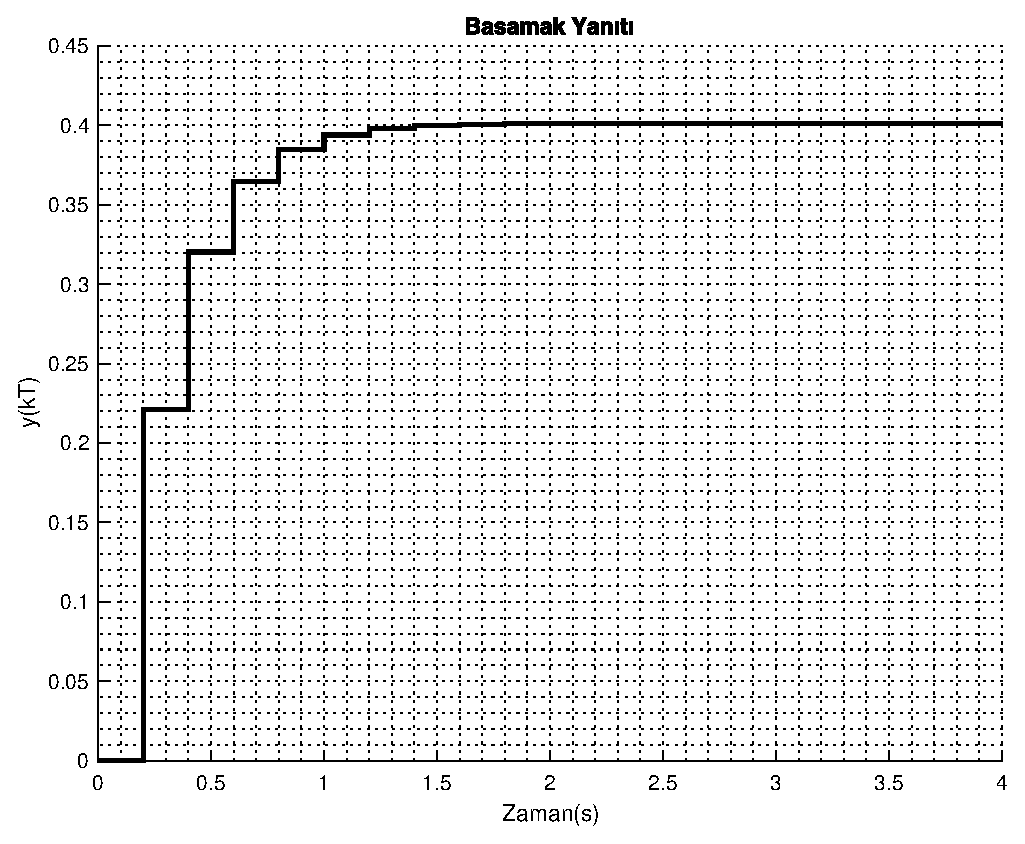
\includegraphics[width=0.75\textwidth]{img/lec6_step1}
    \caption{P kontrol için kapalı çevrim basamak yanıtı}
    \label{fig:lec6_step1}
\end{figure}

PD kontrolör transfer fonksiyonu
\begin{equation}
\begin{split}
    F(z)&=K_p+K_d(1-z^{-1})\\
    &=K_p+K_d(\frac{z-1}{z})\\
    &=\frac{K_pz+K_dz-K_d}{z}\\
    &=\frac{(K_p+K_d)z-K_d}{z}
\end{split}
\end{equation}
olmak üzere kapalı çevrim transfer fonksiyonu
\begin{equation}
    \begin{split}
        T(z)&=\frac{F(z)G(z)}{1+F(z)G(z)}\\
        &=\frac{\frac{(K_p+K_d)z-K_d}{z}\frac{0.1648}{z-0.6703}}{1+\frac{(K_p+K_d)z-K_d}{z}\frac{0.1648}{z-0.6703}}\\
        &=\frac{0.1648(K_d+K_p)z-0.1648-K_d}{z^2+(0.1648(K_p+K_d)-0.6703)z-0.1648K_d}
    \end{split}
\end{equation}
şeklindedir. Bu durumda tasarım problemi
\begin{equation}
    \begin{split}
        0.1648(K_p+K_d)-0.6703&=-0.4144\\
        -0.1648K_d&=0.2019
    \end{split}
\end{equation}
ve çözüm ise $K_d=-1.2251$ ve $K_p=2.7778$ olarak elde edilir. PD kontrolör
\begin{equation}
    F(z)=\frac{1.553 z + 1.225}{z}
\end{equation}
ve kapalı çevrim transfer fonksiyonu ifadesi
\begin{equation}
    T(z)=\frac{0.2559 z + 0.2019}{z^2 - 0.4144 z + 0.2019}
\end{equation}
olarak elde edilir.
\begin{figure}[!htb]
    \centering
    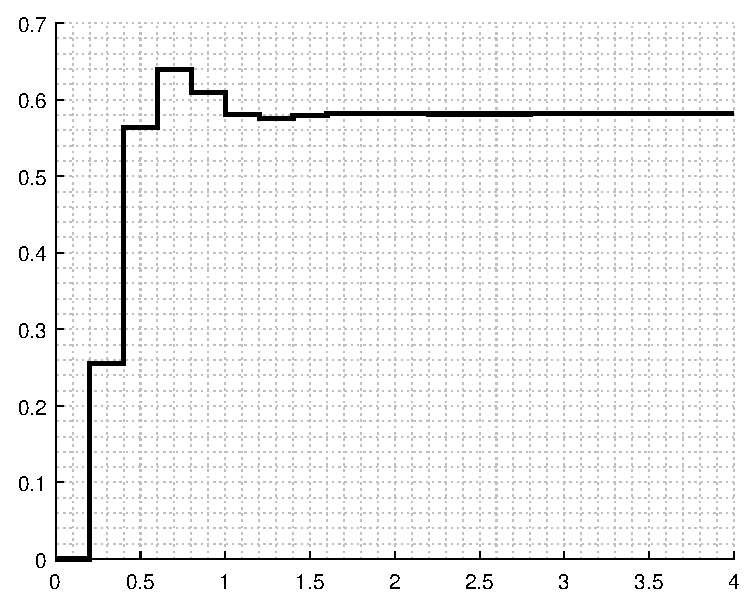
\includegraphics[width=0.75\textwidth]{img/lec6_step2}
    \caption{PD kontrol için kapalı çevrim basamak yanıtı}
    \label{fig:lec6_step2}
\end{figure}

PI kontrolörü 
\begin{equation}
\begin{split}
    F(z)&=K_p+\frac{K_iz}{z-1}\\
    &=\frac{(K_p+K_i)z-K_p}{z-1}
\end{split}
\end{equation}
olarak tanımlanmıştır. Kapalı çevrim transfer fonksiyonu 
\begin{equation}
    \begin{split}
        T(z)&=\frac{F(z)G(z)}{1+F(z)G(z)}\\
        &=\frac{\frac{(K_p+K_i)z-K_p}{z-1}\frac{0.1648}{z-0.6703}}{1+\frac{(K_p+K_i)z-K_p}{z-1}\frac{0.1648}{z-0.6703}}\\
        &=\frac{0.1648(K_p+K_i)z-0.1648K_p}{z^2+(0.1648(K_p+K_i)-1.6703)z+0.6703-0.1648K_p}
    \end{split}
\end{equation}
şeklindedir. Tasarım problemi
\begin{equation}
    \begin{split}
       0.1648(K_p+K_i)-1.6703&=-0.4144\\
       0.6703-0.1648K_p&=0.2019
    \end{split}
\end{equation}
ve çözüm ise $K_p=2.8423$ ve $K_i=4.7784$ şeklindedir. Bu durumda PI kontrolör
\begin{equation}
        F(z)=\frac{7.621 z - 2.842}{z-1}
\end{equation}
ve kapalı çevrim transfer fonksiyonu
\begin{equation}
\begin{split}
    T(z)&=\frac{1.256 z - 0.4685}{z^2 - 0.4141 z + 0.2018}\\
    &=\frac{1.2562 (z-0.373)}{z^2 - 0.4141 z + 0.2018}\\
\end{split}
\end{equation}
olarak elde edilir.

\begin{figure}[!htb]
    \centering
    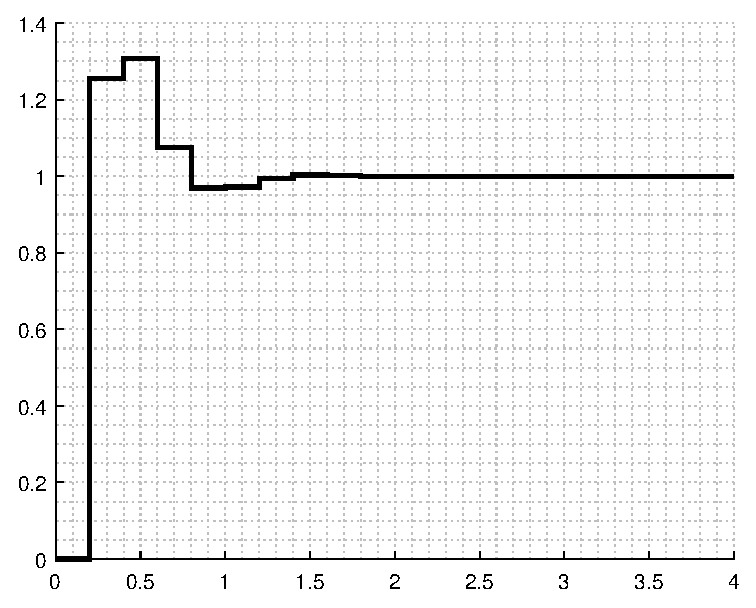
\includegraphics[width=0.75\textwidth]{img/lec6_step3}
    \caption{PI kontrol için kapalı çevrim basamak yanıtı}
    \label{fig:lec6_step3}
\end{figure}

PID kontrolör
\begin{equation}
\begin{split}
    F(z)&=K_p+\frac{K_iz}{z-1}+K_d\frac{z-1}{z}\\
    &=\frac{K_p(z^2-z)+K_iz^2+K_d(z-1)^2}{z^2-z}\\
    &=\frac{K_pz^2-K_pz+K_iz^2+K_dz^2-2K_dz+K_d}{z^2-z}\\
    &=\frac{(K_p+K_i+K_d)z^2-(K_p+2K_d)z+K_d}{z^2-z}
\end{split}
\end{equation}
olarak tanımlanmıştır. Kapalı çevrim transfer fonksiyonu
\begin{equation}
    \begin{split}
        T(z)&=\frac{F(z)G(z)}{1+F(z)G(z)}\\
        &=\frac{\frac{(K_p+K_i+K_d)z^2-(K_p+2K_d)z+K_d}{z^2-z}\frac{0.1648}{z-0.6703}}{1+\frac{(K_p+K_i+K_d)z^2-(K_p+2K_d)z+K_d}{z^2-z}\frac{0.1648}{z-0.6703}}\\
        &=\frac{0.1648((K_p+K_i+K_d)z^2-(K_p+2K_d)z+K_d)}{(z^2-z)(z-0.6703)+0.1648((K_p+K_i+K_d)z^2-(K_p+2K_d)z+K_d)}
    \end{split}
\end{equation}
olmaktadır. Bu durumda tasarım problemi
\begin{equation}
    \begin{split}
        0.1648(K_p+K_i+K_d)-1.6703&= p- 0.4144\\
        0.6703-0.1648(K_p+2K_d)&=0.2019 - 0.4144p\\
        0.1648K_d&=0.2019p
    \end{split}
\end{equation}
olarak verilir. Burada polinom dereceleri eşitlemek amacıyla tasarlanan polinom $s+p$ terimi ile çarpılmıştır. Görüldüğü üzere bilinmeyen sayısı denklem sayısından fazla olması sebebiyle birden çok çözüm bulunmaktadır. Bu durum bir fırsata çevrilirse, isterleri sağlama konusunda bir eniyileştirme işlemi yapılabilir. Bunun için parametrik çözüm elde edilmelidir. $p$, $k_d$ ve $k_i$ kalan parametre $k_p$ cinsinden elde edilirse 
\begin{equation}
    \begin{split}
        p&=15.51k_p-44.08\\
        k_d&=19k_p-54\\
        k_i&=74.1k_p-205.8
    \end{split}
\end{equation}
olarak bulunur. Kapalı çevrim sistemin kararlılığı açısından $|p|<1$ şartı sağlanmalıdır. Bu sebeple $k_p$ için sınır değerler
\begin{equation}
    15.51k_p-44.08=1,\quad 15.51k_p-44.08=-1
\end{equation}
denklemleri çözülerek 
\begin{equation}
    2.7778<k_p<2.9067
\end{equation}
elde edilir. Bu aralıkta değerler tek tek seçilir ve kapalı çevrim transfer fonksiyonu ve elde edilen yerleşme zamanı ve aşım verileri ile 
\begin{equation}
    J(k_p)=\frac{|t_s-1|}{2}+\frac{|os-10|}{20}
\end{equation}
amaç fonksiyonunda yerine yazılır. $J(k_p)$'yi en az yapan $k_p$ değeri $k_p=2.7998$ olarak elde edilir. Bu durumda kontrolör parametreleri $k_d=-0.8067$ ve $k_i=1.6319$ ve dolayısıyla kontrolör transfer fonksiyonu
\begin{equation}
    F(z)=\frac{3.625 z^2 - 1.186 z - 0.8067}{ z^2 - z}
\end{equation}
şeklindedir. Kapalı çevrim transfer fonksiyonu 
\begin{equation}
\begin{split}
    T(z)&=\frac{0.5975 z^2 - 0.1956 z - 0.133}{z^3 - 1.073 z^2 + 0.4748 z - 0.133}\\
    &=\frac{0.59754 (z-0.663) (z+0.3357)}{(z-0.6585) (z^2 - 0.4143z + 0.2019)}\\
    &\approx\frac{0.6014(z+0.3357)}{z^2 - 0.4143z + 0.2019}
\end{split}
\end{equation}
olarak hesaplanmaktadır. Görüldüğü üzere yakın bir kutup ve sıfır mevcuttur. Bu yakınlık bir götürmeye sebep olarak istenen kutup dağılımına daha yakın bir kapalı çevrim sistem elde edilmektedir. Basamak yanıtı Şekil~\ref{fig:lec6_step4} ile verilmiştir.

\begin{figure}[!htb]
    \centering
    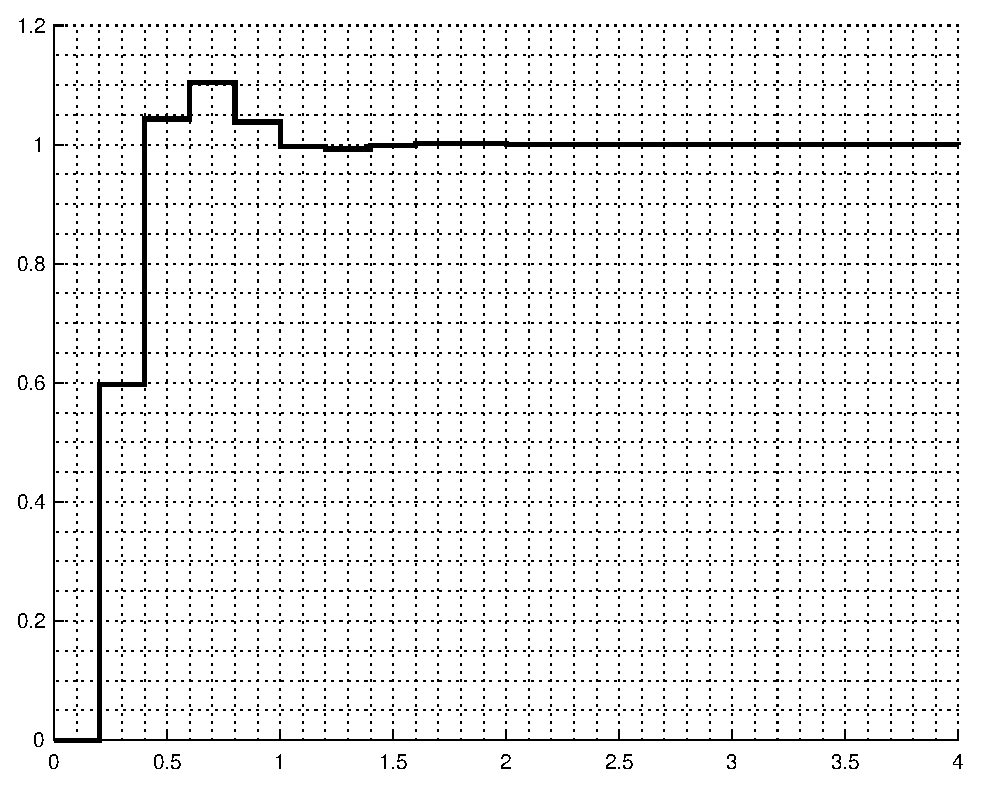
\includegraphics[width=0.75\textwidth]{img/lec6_step4}
    \caption{PID kontrol için kapalı çevrim basamak yanıtı}
    \label{fig:lec6_step4}
\end{figure}

Görüldüğü üzere isterlere oldukça yakın değerler elde edilmiştir. Bunun sebebi, PID kontrolörün fazladan parametreye sahip olması ve bu parametre kullanılarak bir eniyileştirme işleminin mümkün olmasıdır.
\chapter{Z Tanım Bölgesinde P Kontrolör Tasarımı}
\begin{enumerate}
    \item Geçici hal yanıtını şekillendirecek isterler dikkate alınarak s tanım bölgesinde baskın kutuplar seçilir. 
    \item Baskın kutuplar $z=e^{sT}$ ilişkisi ile z tanım bölgesine aktarılır. 
    \item Kontrol edilecek sistem Z tanım bölgesine geçirilir. 
    \item Kapalı çevrim transfer fonksiyonu elde edilir ve kutup atama yapılır.
\end{enumerate}
Örnek sistem
\begin{equation}
    G(s)=\frac{1}{s+2}
\end{equation}
z tanım bölgesinde $T=0.2$ olmak üzere
\begin{equation}
    G(z)=\frac{0.1648}{z-0.6703}
\end{equation}
olarak elde edilmektedir. Yerleşme zamanı $t_s=2$ ve aşım $\%10$ isterleri verilmiştir. Bu durumda $\zeta=0.591$ ve $w_n=6.7664$ seçilir. Seçilen sönüm oranı ve doğal frekans ile baskın kutuplar
\begin{equation}
    s_{1,2}=-4 \pm 5.4575i
\end{equation}
şeklinde hesaplanır. $z=e^{sT}$ ifadesi ile z tanım bölgesinde kutuplar
\begin{equation}
    z_{1,2}=0.2072 \pm 0.3987i
\end{equation}
ve kutuplardan oluşturulacak polinom
\begin{equation}
    p(z)=z^2-0.4144 z+0.2019
\end{equation}
olarak hesaplanır. P tipi kontrolör ile kapalı çevrim transfer fonksiyonunun ifadesi
\begin{equation}
\begin{split}
    T(z)&=\frac{kG(z)}{1+kG(z)}\\
    &=\frac{k\frac{0.1648}{z-0.6703}}{1+k\frac{0.1648}{z-0.6703}}\\
    &=\frac{k(0.1648)}{z-0.6703+k(0.1648)}\\
    &=\frac{0.1648k}{z+0.1648k-0.6703}
\end{split}
\end{equation}
şeklindedir. Görüldüğü üzere karakteristik polinom birinci dereceden elde edilmiştir ve her iki isterlerin sağlanması mümkün değildir. Yerleşme zamanı sağlanmak istenirse,
\begin{equation}
    s=-\frac{4}{t_s}=-4
\end{equation}
ve z tanım bölgesinde
\begin{equation}
    z=e^{sT}=e^{-0.8}=0.4493
\end{equation}
elde edilir. Bu durumda P kontrolör
\begin{equation}
\begin{split}
    -0.1648k+0.6703&=0.4493\\
    k&=1.341
\end{split}
\end{equation}
şeklindedir. Kapalı çevrim transfer fonksiyonu
\begin{equation}
    T(z)=\frac{0.221}{z - 0.4493}
\end{equation}
şeklindedir.
\begin{figure}[!htb]
    \centering
    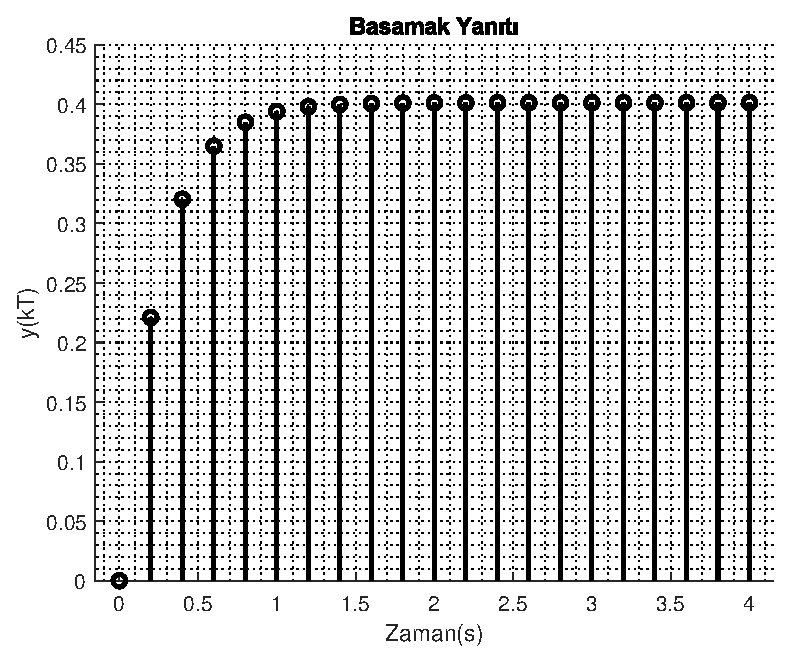
\includegraphics[width=0.75\textwidth]{img/lec7_step1}
    \caption{P kontrol için kapalı çevrim basamak yanıtı ($k=1.341$)}
    \label{fig:lec7_step1}
\end{figure}

\begin{figure}[!htb]
    \centering
    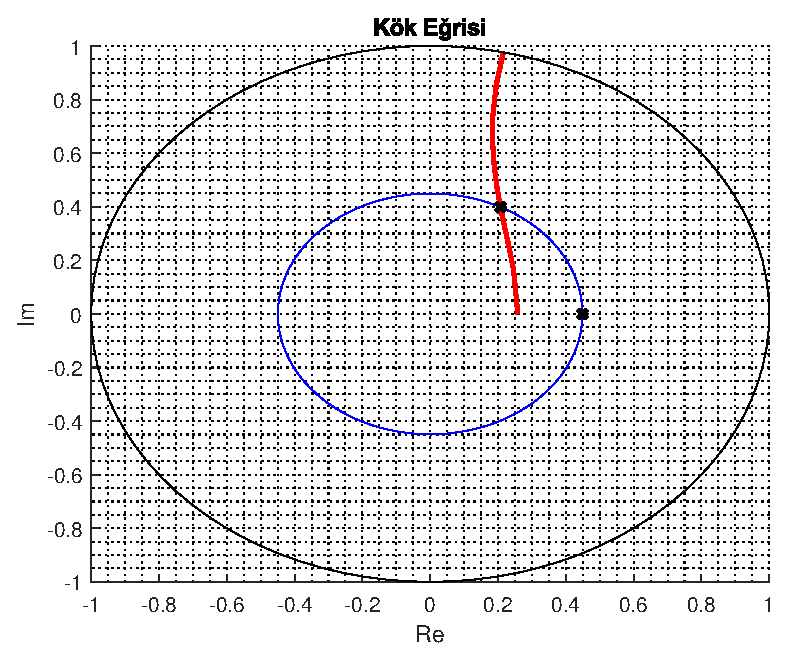
\includegraphics[width=0.75\textwidth]{img/lec7_rlocus1}
    \caption{P kontrol için kök eğrisi}
    \label{fig:lec7_rlocus1}
\end{figure}
Tasarıma ait kök eğrisi Şekil~\ref{fig:lec7_rlocus1} ile verilmiştir. Seçilen $w_n$ değerine karşılık değişken $\zeta$ değeri için eğri gösterilmiştir ve belirli bir aşıma karşılık düşen $\zeta$ değeri için tasarım noktası gösterilmiştir. Bu nokta yerleşme zamanı isteri ile elde edilen yarıçaplı çember üzerindedir. Dikkat edilirse tasarımda $\zeta$ parametresi kullanılamamıştır, çünkü kapalı çevrim karakteristik polinomunun derecesi yetersiz kalmıştır. Sadece yerleşme zamanını karşılayacak gerçel bir kutup seçilebilmektedir ve bu z tanım bölgesinde Şekil~\ref{fig:lec7_rlocus1}'deki kök eğrisinde gösterilen çembere karşılık düşmektedir. Tasarlanan P kontrolörün Kapalı çevrim transfer fonksiyonuna ait basamak yanıtı Şekil~\ref{fig:lec7_step1} ile verilmiştir. Görüldüğü üzere aşım yapmayan fakat yerleşme zamanı isterini karşılayan bir yanıt elde edilmiştir. Ayrıca, tasarım giriş sinyalini belirli bir hata ile izlemektedir.

P kontrolör için bir diğer alternatif ise 
\begin{equation}
\begin{split}
    -0.1648k+0.6703&=-0.4493\\
    k&=6.7937
\end{split}
\end{equation}
şeklindedir ve kapalı çevrim transfer fonksiyonu
\begin{equation}
    T(z)=\frac{1.1199}{z + 0.4496}
\end{equation}
şeklindedir. Basamak yanıtı Şekil~\ref{fig:lec7_step2}'de verilmiştir.

\begin{figure}[!htb]
    \centering
    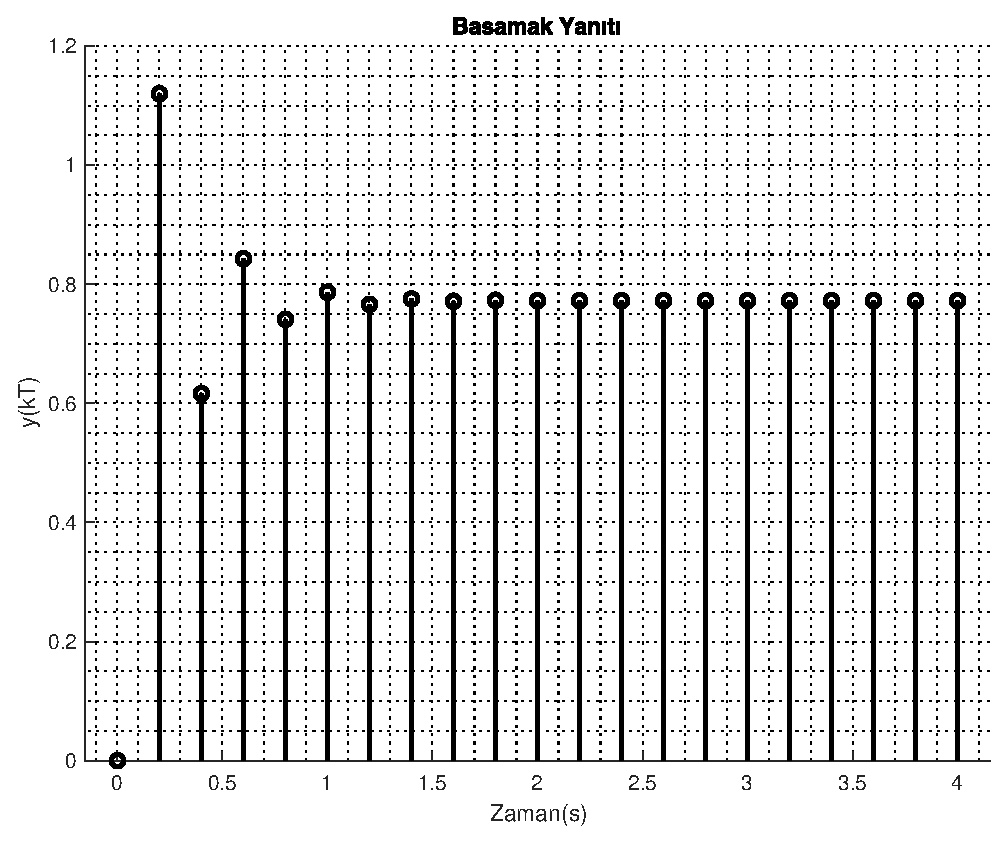
\includegraphics[width=0.75\textwidth]{img/lec7_step2}
    \caption{P kontrol için kapalı çevrim basamak yanıtı($k=6.7937$)}
    \label{fig:lec7_step2}
\end{figure}

$z=-0.4496$ çözümü için s tanım bölgesine dönüşüm sonucu
\begin{equation}
\begin{split}
    z&=e^{0.2s}\\
    s&=\frac{\log{z}}{0.2}\\
    s&=5\log{(-0.4496)}\\
    s&=-3.9970 +15.7080i
\end{split}
\end{equation}
elde edilir. Sönüm oranı $\zeta$
\begin{equation}
    \begin{split}
        \theta&=\tan^{-1}\left(\frac{15.708}{3.997}\right)\\
        \theta&=75.7237^o\\
        \zeta&=\cos(\theta)\\
        \zeta&=0.2466
    \end{split}
\end{equation}
olarak hesaplanır ve aşım
\begin{equation}
        100e^{\frac{-\pi \zeta}{\sqrt{1-\zeta^2}}}=\%44.96
\end{equation}
olarak elde edilir. Birinci dereceden bir sistem s tanım bölgesinde aşım yapamazken bu durum z tanım bölgesinde geçerli değildir. Sistem kutupları s tanım bölgesinde gerçel olmak durumundadır, fakat z tanım bölgesinde bir kutup negatif gerçel olması sonucu tanım bölgesinde karmaşık sayıya karşılık düşmektedir. Bu sebeple z tanım bölgesinde aşım yapabilir. 

\chapter{Z Tanım Bölgesinde PD Kontrolör Tasarımı}
\begin{enumerate}
    \item Geçici hal yanıtını şekillendirecek isterler dikkate alınarak s tanım bölgesinde baskın kutuplar seçilir. 
    \item Baskın kutuplar $z=e^{sT}$ ilişkisi ile z tanım bölgesine aktarılır. 
    \item Kontrol edilecek sistem Z tanım bölgesine geçirilir. 
    \item Kapalı çevrim transfer fonksiyonu elde edilir ve kutup atama yapılır.
\end{enumerate}
Örnek sistem
\begin{equation}
    G(s)=\frac{1}{s+2}
\end{equation}
z tanım bölgesinde $T=0.2$ olmak üzere
\begin{equation}
    G(z)=\frac{0.1648}{z-0.6703}
\end{equation}
olarak elde edilmektedir. Yerleşme zamanı $t_s=2$ ve aşım $\%10$ isterleri verilmiştir. Bu durumda $\zeta=0.591$ ve $w_n=6.7664$ seçilir. Seçilen sönüm oranı ve doğal frekans ile baskın kutuplar
\begin{equation}
    s_{1,2}=-4 \pm 5.4575i
\end{equation}
şeklinde hesaplanır. $z=e^{sT}$ ifadesi ile z tanım bölgesinde kutuplar
\begin{equation}
    z_{1,2}=0.2072 \pm 0.3987i
\end{equation}
ve kutuplardan oluşturulacak polinom
\begin{equation}
    p(z)=z^2-0.4144 z+0.2019
\end{equation}
olarak hesaplanır. P tipi kontrolör ile kapalı çevrim transfer fonksiyonunun ifadesi
\begin{equation}
\begin{split}
    T(z)&=\frac{kG(z)}{1+kG(z)}\\
    &=\frac{k\frac{0.1648}{z-0.6703}}{1+k\frac{0.1648}{z-0.6703}}\\
    &=\frac{k(0.1648)}{z-0.6703+k(0.1648)}\\
    &=\frac{0.1648k}{z+0.1648k-0.6703}
\end{split}
\end{equation}
şeklindedir. Görüldüğü üzere karakteristik polinom birinci dereceden elde edilmiştir ve her iki isterlerin sağlanması mümkün değildir. Yerleşme zamanı sağlanmak istenirse,
\begin{equation}
    s=-\frac{4}{t_s}=-4
\end{equation}
ve z tanım bölgesinde
\begin{equation}
    z=e^{sT}=e^{-0.8}=0.4493
\end{equation}
elde edilir. PD kontrolör transfer fonksiyonu
\begin{equation}
\begin{split}
    F(z)&=K_p+K_d(1-z^{-1})\\
    &=K_p+K_d(\frac{z-1}{z})\\
    &=\frac{K_pz+K_dz-K_d}{z}\\
    &=\frac{(K_p+K_d)z-K_d}{z}
\end{split}
\end{equation}
olmak üzere kapalı çevrim transfer fonksiyonu
\begin{equation}
    \begin{split}
        T(z)&=\frac{F(z)G(z)}{1+F(z)G(z)}\\
        &=\frac{\frac{(K_p+K_d)z-K_d}{z}\frac{0.1648}{z-0.6703}}{1+\frac{(K_p+K_d)z-K_d}{z}\frac{0.1648}{z-0.6703}}\\
        &=\frac{0.1648(K_d+K_p)z-0.1648-K_d}{z^2+(0.1648(K_p+K_d)-0.6703)z-0.1648K_d}
    \end{split}
\end{equation}
şeklindedir. Bu durumda tasarım problemi
\begin{equation}
    \begin{split}
        0.1648(K_p+K_d)-0.6703&=-0.4144\\
        -0.1648K_d&=0.2019
    \end{split}
\end{equation}
ve çözüm ise $K_d=-1.2251$ ve $K_p=2.7778$ olarak elde edilir. PD kontrolör
\begin{equation}
    F(z)=\frac{1.553 z + 1.225}{z}
\end{equation}
ve kapalı çevrim transfer fonksiyonu ifadesi
\begin{equation}
    T(z)=\frac{0.2559 z + 0.2019}{z^2 - 0.4144 z + 0.2019}
\end{equation}
olarak elde edilir.
% \begin{figure}[!htb]
%     \centering
%     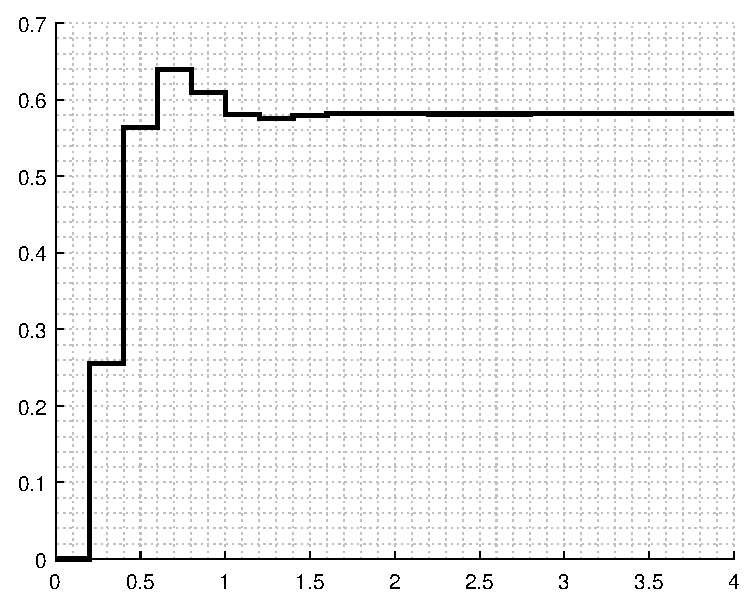
\includegraphics[width=0.75\textwidth]{img/lec6_step2}
%     \caption{PD kontrol için kapalı çevrim basamak yanıtı}
%     \label{fig:lec6_step2}
% \end{figure}

\documentclass[12pt,hyperref=unicode]{beamer}

\usepackage[utf8]{inputenc}
\usepackage[turkish]{babel}
\usepackage[T1]{fontenc}

\usepackage{amsmath}
\usepackage{amssymb}
\usepackage{amsthm}
\usepackage{enumerate}
\usepackage{tikz}
\usepackage{transparent}
\usepackage{xcolor}
\usepackage{listings}
\usepackage{verbatim}
\usepackage{graphicx}

\usepackage{pgfplots}

\usetheme{Warsaw}
\usecolortheme{default}
\definecolor{nigdeyesili_acik}{RGB}{3, 150, 166}
\definecolor{nigdeyesili_koyu}{RGB}{143, 209, 217}
\setbeamercolor{structure}{fg=nigdeyesili_acik}

\author[Dr. Mehmet CANEVİ]{Arş.~Gör.~Dr.~M.~Canevi\inst{1}}

\institute{
    \inst{1}%
    Bilgisayar Mühendisliği\\
    Mühendislik Fakültesi
}
    
\date[2025] {Ders Notları, Ocak 2025}
\setbeamertemplate{footline}[frame number]

\logo{\transparent{0.4}
\includegraphics[width = 20mm]{logo}}

\definecolor{mGreen}{rgb}{0,0.6,0}
\definecolor{mGray}{rgb}{0.5,0.5,0.5}
\definecolor{mPurple}{rgb}{0.58,0,0.82}
\definecolor{backgroundColour}{rgb}{0.95,0.95,0.92}

\lstloadlanguages{C}
\lstdefinestyle{CStyle}{
    backgroundcolor=\color{backgroundColour},   
    commentstyle=\color{mGreen},
    keywordstyle=\color{red},
    numberstyle=\tiny\color{mGray},
    stringstyle=\color{mGreen},
    basicstyle=\footnotesize,
    breakatwhitespace=false,         
    breaklines=true,                 
    captionpos=b,                    
    keepspaces=true,                 
    numbers=left,                    
    numbersep=2pt,                  
    showspaces=false,                
    showstringspaces=false,
    showtabs=false,                  
    tabsize=1,
    language=C
}
\lstset{style=CStyle}

\AtBeginDocument{\shorthandoff{=}}
\title[Ders 9] {P-tipi kontrolör I (Kuram)}
\begin{document}
%%%%%%%%%%%%%%%%%%%%%%%%%%%%%%%%%%%%%%%%%%%%%%%%%%%%%%%%%%%%%%%%%%%%%%%%%%%%%%%%
\frame{\titlepage}
\begin{frame}[fragile]{İçidekiler}
    \tableofcontents
\end{frame}
%%%%%%%%%%%%%%%%%%%%%%%%%%%%%%%%%%%%%%%%%%%%%%%%%%%%%%%%%%%%%%%%%%%%%%%%%%%%%%%%
\section{P-tipi kontrolör}
\begin{frame}[fragile]{Sistem}
    a
\end{frame}
%%%%%%%%%%%%%%%%%%%%%%%%%%%%%%%%%%%%%%%%%%%%%%%%%%%%%%%%%%%%%%%%%%%%%%%%%%%%%%%%
\end{document}
\chapter{Z Tanım Bölgesinde PID Kontrolör Tasarımı}
Örnek sistem
\begin{equation}
    G(s)=\frac{1}{s+2}
\end{equation}
z tanım bölgesinde $T=0.2$ olmak üzere
\begin{equation}
    G(z)=\frac{0.1648}{z-0.6703}
\end{equation}
olarak elde edilmektedir. Yerleşme zamanı $t_s=1$ ve aşım $\%10$ isterleri verilmiştir. Bu durumda $\zeta=0.591$ ve $w_n=6.7664$ seçilir. Seçilen sönüm oranı ve doğal frekans ile baskın kutuplar
\begin{equation}
    s_{1,2}=-4 \pm 5.4575i
\end{equation}
şeklinde hesaplanır. $z=e^{sT}$ ifadesi ile z tanım bölgesinde kutuplar
\begin{equation}
    z_{1,2}=0.2072 \pm 0.3987i
\end{equation}
ve kutuplardan oluşturulacak polinom
\begin{equation}
    p(z)=z^2-0.4144 z+0.2019
\end{equation}
olarak hesaplanır. PID kontrolör
\begin{equation}
\begin{split}
    F(z)&=K_p+\frac{K_iz}{z-1}+K_d\frac{z-1}{z}\\
    &=\frac{K_p(z^2-z)+K_iz^2+K_d(z-1)^2}{z^2-z}\\
    &=\frac{K_pz^2-K_pz+K_iz^2+K_dz^2-2K_dz+K_d}{z^2-z}\\
    &=\frac{(K_p+K_i+K_d)z^2-(K_p+2K_d)z+K_d}{z^2-z}
\end{split}
\end{equation}
olarak tanımlanmıştır. Kapalı çevrim transfer fonksiyonu
\begin{equation}
    \begin{split}
        T(z)&=\frac{F(z)G(z)}{1+F(z)G(z)}\\
        &=\frac{\frac{(K_p+K_i+K_d)z^2-(K_p+2K_d)z+K_d}{z^2-z}\frac{0.1648}{z-0.6703}}{1+\frac{(K_p+K_i+K_d)z^2-(K_p+2K_d)z+K_d}{z^2-z}\frac{0.1648}{z-0.6703}}\\
        &=\frac{0.1648((K_p+K_i+K_d)z^2-(K_p+2K_d)z+K_d)}{(z^2-z)(z-0.6703)+0.1648((K_p+K_i+K_d)z^2-(K_p+2K_d)z+K_d)}
    \end{split}
\end{equation}
olmaktadır. Bu durumda tasarım problemi
\begin{equation}
    \begin{split}
        0.1648(K_p+K_i+K_d)-1.6703&= p- 0.4144\\
        0.6703-0.1648(K_p+2K_d)&=0.2019 - 0.4144p\\
        0.1648K_d&=0.2019p
    \end{split}
\end{equation}
olarak verilir. Burada polinom dereceleri eşitlemek amacıyla tasarlanan polinom $s+p$ terimi ile çarpılmıştır. Görüldüğü üzere bilinmeyen sayısı denklem sayısından fazla olması sebebiyle birden çok çözüm bulunmaktadır. Bu durum bir fırsata çevrilirse, isterleri sağlama konusunda bir eniyileştirme işlemi yapılabilir. Bunun için parametrik çözüm elde edilmelidir. $p$, $k_d$ ve $k_i$ kalan parametre $k_p$ cinsinden elde edilirse 
\begin{equation}
    \begin{split}
        p&=15.51k_p-44.08\\
        k_d&=19k_p-54\\
        k_i&=74.1k_p-205.8
    \end{split}
\end{equation}
olarak bulunur. Kapalı çevrim sistemin kararlılığı açısından $|p|<1$ şartı sağlanmalıdır. Bu sebeple $k_p$ için sınır değerler
\begin{equation}
    15.51k_p-44.08=1,\quad 15.51k_p-44.08=-1
\end{equation}
denklemleri çözülerek 
\begin{equation}
    2.7778<k_p<2.9067
\end{equation}
elde edilir. Bu aralıkta değerler tek tek seçilir ve kapalı çevrim transfer fonksiyonu ve elde edilen yerleşme zamanı ve aşım verileri ile 
\begin{equation}
    J(k_p)=\frac{|t_s-1|}{2}+\frac{|os-10|}{20}
\end{equation}
amaç fonksiyonunda yerine yazılır. $J(k_p)$'yi en az yapan $k_p$ değeri $k_p=2.7998$ olarak elde edilir. Bu durumda kontrolör parametreleri $k_d=-0.8067$ ve $k_i=1.6319$ ve dolayısıyla kontrolör transfer fonksiyonu
\begin{equation}
    F(z)=\frac{3.625 z^2 - 1.186 z - 0.8067}{ z^2 - z}
\end{equation}
şeklindedir. Kapalı çevrim transfer fonksiyonu 
\begin{equation}
\begin{split}
    T(z)&=\frac{0.5975 z^2 - 0.1956 z - 0.133}{z^3 - 1.073 z^2 + 0.4748 z - 0.133}\\
    &=\frac{0.59754 (z-0.663) (z+0.3357)}{(z-0.6585) (z^2 - 0.4143z + 0.2019)}\\
    &\approx\frac{0.6014(z+0.3357)}{z^2 - 0.4143z + 0.2019}
\end{split}
\end{equation}
olarak hesaplanmaktadır. Görüldüğü üzere yakın bir kutup ve sıfır mevcuttur. Bu yakınlık bir götürmeye sebep olarak istenen kutup dağılımına daha yakın bir kapalı çevrim sistem elde edilmektedir. Basamak yanıtı Şekil~\ref{fig:lec10_step1} ile verilmiştir.

\begin{figure}[!htb]
    \centering
    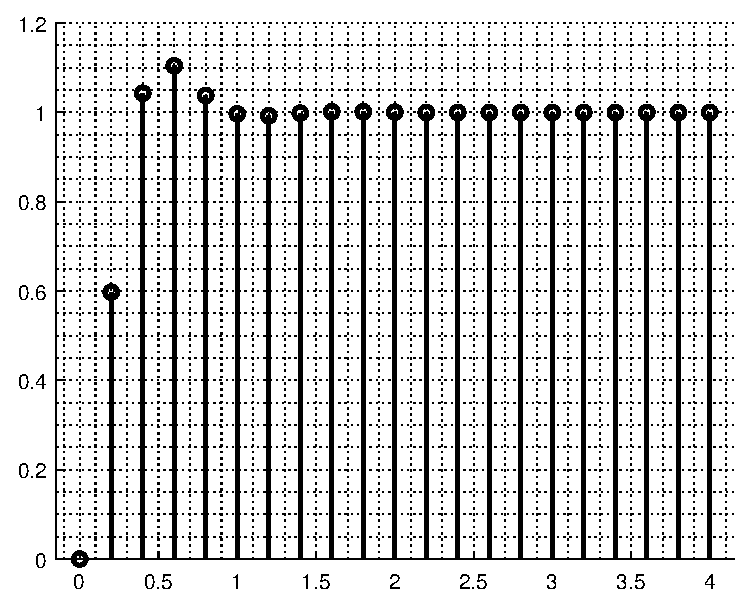
\includegraphics[width=0.75\textwidth]{img/lec10_step1}
    \caption{PID kontrol için kapalı çevrim basamak yanıtı}
    \label{fig:lec10_step1}
\end{figure}

Görüldüğü üzere isterlere oldukça yakın değerler elde edilmiştir. Bunun sebebi, PID kontrolörün fazladan parametreye sahip olması ve bu parametre kullanılarak bir eniyileştirme işleminin mümkün olmasıdır.
\chapter{Z Tanım Bölgesinde Durum Uzayı}

\chapter{Z Tanım Bölgesinde Durum Geri Besleme Kontrolörü}
Durum uzay modeli
\begin{equation}
    x(k)=A x(k-1)+Bu(k-1),\quad y(k-1)=C x(k-1)
\end{equation}
olmak üzere 
\begin{equation}
    u(k-1)=K x(k-1)
\end{equation}
kontrolörüne \textbf{Durum Geri Besleme} kontrolörü adı verilmektedir. Dikkat edilirse bu kontrol kuralı
\begin{equation}
\begin{split}
    u(k-1)&=K x(k-1)\\
    u(k-1)&=\begin{bmatrix}k_1& k_2& \cdots& k_n\end{bmatrix} \begin{bmatrix}x_1(k-1)\\x_2(k-1)\\\vdots\\x_n(k-1)\end{bmatrix}\\
    u(k-1)&=k_1x_1(k-1)+k_2x_2(k-1)+\cdots+k_nx_n(k-1)
\end{split}
\end{equation}
olarak yazılabilir. Bu kontrolör ile kapalı çevrim durum uzay modeli
\begin{equation}
    \begin{split}
        x(k)&=A x(k-1)+Bu(k-1),\quad y(k-1)=C x(k-1)\\
        x(k)&=A x(k-1)+BKx(k-1),\quad y(k-1)=C x(k-1)\\
        x(k)&=(A+BK) x(k-1),\quad y(k-1)=C x(k-1)
    \end{split}
\end{equation}
olarak elde edilir. Kapalı çevrim modelin z tanım bölgesi ifadesi
\begin{equation}
    \begin{split}
        x(k)&=(A+BK) x(k-1)+B r(k-1),\quad y(k-1)=C x(k-1)\\
        z^1 x(k-1)&=(A+BK) x(k-1)+B r(k-1),\quad y(k-1)=C x(k-1)\\
        (zI-(A+BK)) x(k-1)&=B r(k-1),\quad y(k-1)=C x(k-1)\\
        x(k-1)&=(zI-(A+BK))^{-1} B r(k-1),\quad y(k-1)=C x(k-1)\\
        y(k-1)&=C(zI-(A+BK))^{-1}B r(k-1)\\
        \frac{y(k-1)}{r(k-1)}&=C(zI-(A+BK))^{-1}B
    \end{split}
\end{equation}
şeklindedir ve karakteristik polinom
\begin{equation}
    \begin{split}
        p_c(z)=det(zI-(A+BK))
    \end{split}
\end{equation}
ile hesaplanır.


\chapter{Z Tanım Bölgesinde Luenberger Gözleyicisi}
Durum uzay modeli
\begin{equation}
    x(k)=A x(k-1)+Bu(k-1),\quad y(k-1)=C x(k-1)
\end{equation}
olmak üzere \textbf{Luenberger Gözleyicisi}
\begin{equation}
    \hat{x}(k)=A \hat{x}(k-1)+Bu(k-1)+L(y(k-1)-\hat{y}(k-1)),\quad \hat{y}(k-1)=C \hat{x}(k-1)
\end{equation}
olarak tanımlanmaktadır. Burada sistem modelinin bir benzeri kullanılmaktadır, fakat ek bir terim olarak sistem çıkışı ve gözleyici çıkışı farkının $L$ terimi ile çarpımı gözleyici durumlarına etki etmektedir. Bu etkinin seçilmesine gözleyici tasarımı denmektedir. Gözleyicinin amacı sistem durumlarını hesaplamaktır. Bu sebeple sistem durumları ve gözleyici durumları arasındaki fark, veya hata, $e(k)$ olmak üzere
\begin{equation}
    e(k)=x(k)-\hat{x}(k)
\end{equation}
olarak tanımlanır. Hatanın değişimi ise $\Delta e(k)$ olmak üzere,
\begin{equation}
\begin{split}
    \Delta e(k)&=\Delta (x(k)-\hat{x}(k))\\
    &=\Delta x(k)-\Delta\hat{x}(k)\\
    &=\frac{x(k)-x(k-1)}{T}-\frac{\hat{x}(k)-\hat{x}(k-1)}{T}\\
    &=\frac{A x(k-1)-x(k-1)-A\hat{x}(k-1)-L(y(k-1)-\hat{y}(k-1))+\hat{x}(k-1)}{T}\\
    &=\frac{A e(k-1)-e(k-1)-LC(x(k-1)-\hat{x}(k-1))}{T}\\
    &=\frac{A e(k-1)-e(k-1)-LCe(k-1)}{T}\\
    e(k)-e(k-1)&=(A-LC-I)e(k-1)\\
    e(k)&=(A-LC)e(k-1)
\end{split}
\end{equation}
elde edilir. Elde edilen sistemin kararlı kılınması durumunda 
\begin{equation}
\begin{split}
    e(k)&\rightarrow 0\\
    x(k)-\hat{x}(k)&\rightarrow 0\\
    x(k)&\rightarrow \hat{x}(k)
\end{split}
\end{equation}
olacağından, gözleyici çalışacaktır. Bunun için,
\begin{equation}
    p_c(s)=det(sI-(A-LC))
\end{equation}
ile elde edilen polinomun kutuplarının kararlı olacak şekilde seçilmesi gerekmektedir. Gözleyici katsayısı $L$ 
\begin{equation}
    L=p_d(A)\begin{bmatrix}C\\ CA\\ \vdots\\ CA^{n-1}\end{bmatrix}^{-1}\begin{bmatrix}0\\ 0\\ \vdots\\ 0\\ 1\end{bmatrix}
\end{equation}
ile seçilebilmektedir. Örnek olarak
\begin{equation}
    \begin{split}
\begin{bmatrix}
    x_1[k]\\
    x_2[k]
\end{bmatrix}&=
\begin{bmatrix}
    1& 0.1\\
    -0.1& 0.95
\end{bmatrix}\begin{bmatrix}
    x_1[k-1]\\
    x_2[k-1]
\end{bmatrix}+\begin{bmatrix}
    0\\
    0.1
\end{bmatrix}u[k-1]\\
y[k-1]&=\begin{bmatrix}
    1&0 
\end{bmatrix}\begin{bmatrix}
    x_1[k-1]\\
    x_2[k-1]
\end{bmatrix}\\
\end{split}
\end{equation}
ile verilen sistem için gözleyici katsayısı
\begin{equation}
\begin{split}
    L&=p_d(A)\begin{bmatrix}C\\ CA\\ \vdots\\ CA^{n-1}\end{bmatrix}^{-1}\begin{bmatrix}0\\ 0\\ \vdots\\ 0\\ 1\end{bmatrix}\\
    &=\begin{bmatrix} 0.8&0.1750\\-0.175&0.7125\end{bmatrix}
    \begin{bmatrix} 1&0\\1&0.1\end{bmatrix}^{-1}\begin{bmatrix}0\\ 1\end{bmatrix}\\
    &=\begin{bmatrix}1.75\\7.125\end{bmatrix}
\end{split}
\end{equation}
olarak hesaplamaktır. Elde edilen Luenberger gözleyicisi Şekil~\ref{fig:lec13_model1} ile gösterilmektedir.

\begin{figure}[!htb]
    \centering
    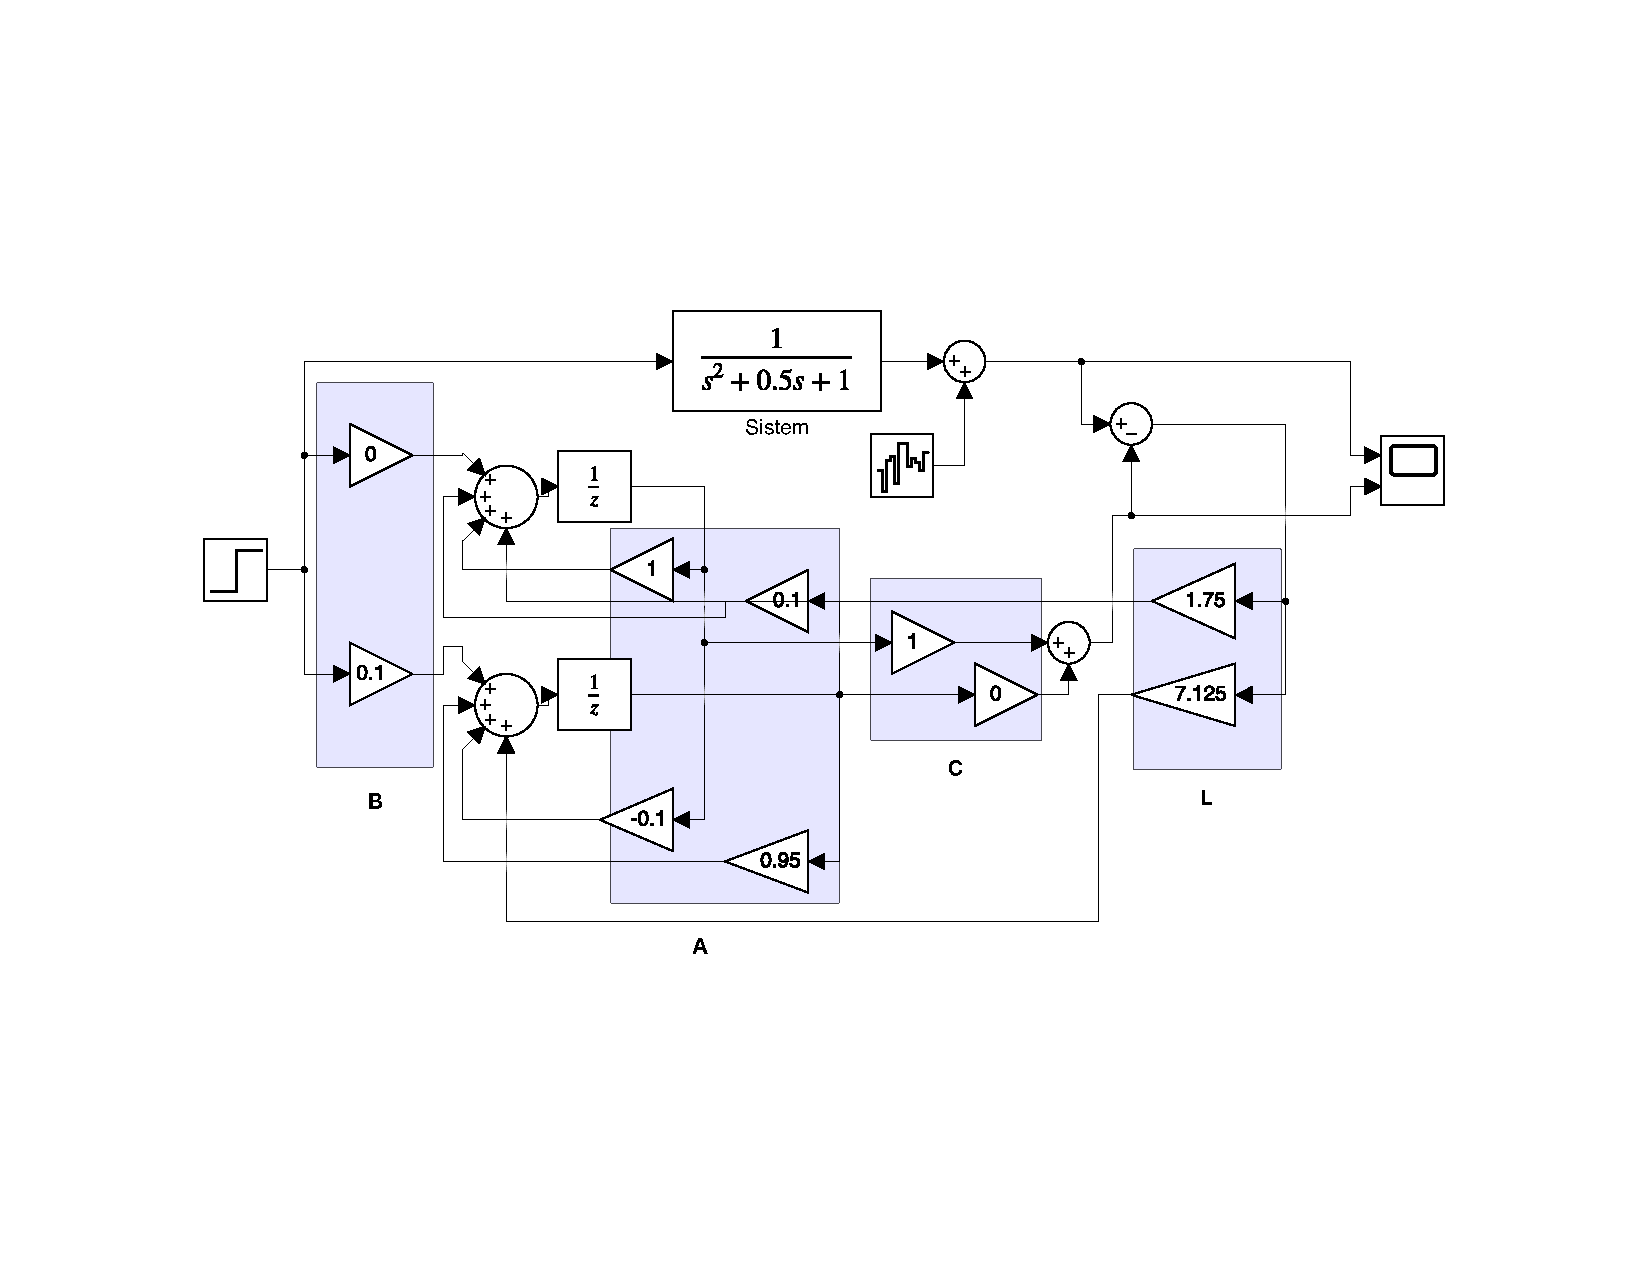
\includegraphics[width=\textwidth]{img/lec13_model1}
    \caption{Yay-kütle-damper sistemine ait gözleyici}
    \label{fig:lec13_model1}
\end{figure}

\begin{figure}[!htb]
    \centering
    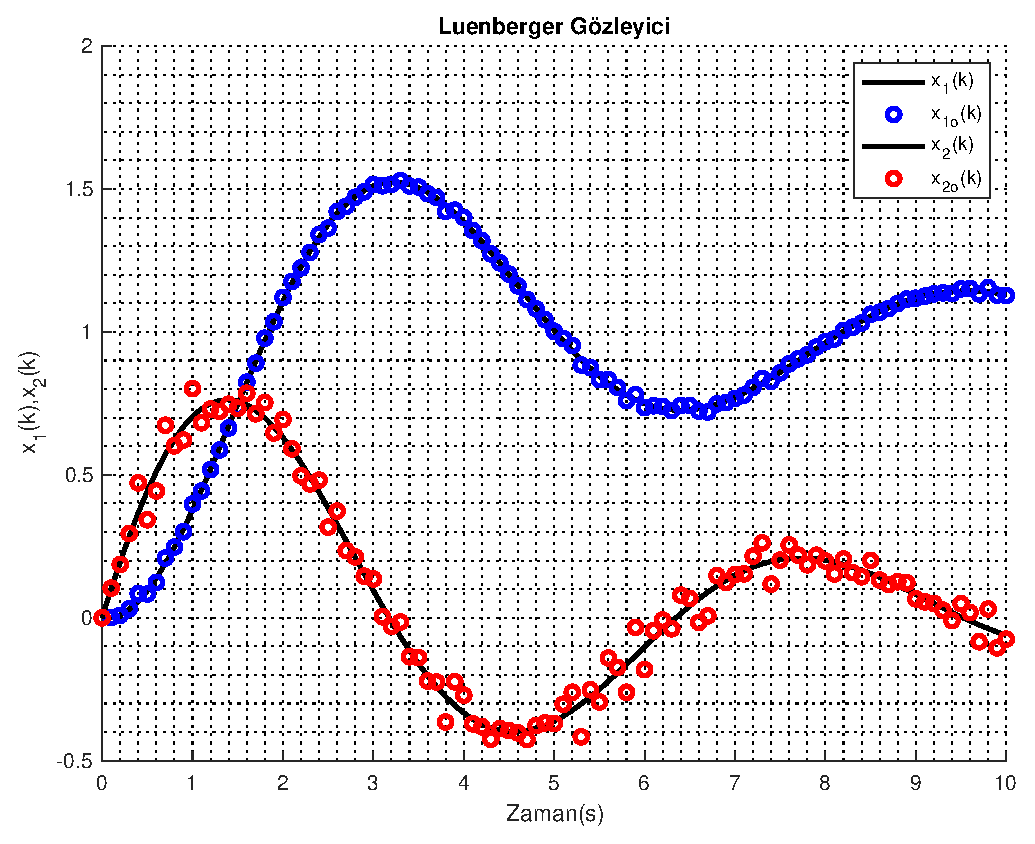
\includegraphics[width=0.75\textwidth]{img/lec13_plot1}
    \caption{Yay-kütle-damper sistemine ait gözleyici yanıtı}
    \label{fig:lec13_plot1}
\end{figure}

\end{document}
